\documentclass[10pt, aspectratio=169]{beamer}

\usepackage[utf8]{inputenc}
\usepackage[T1]{fontenc}
\usepackage[english]{babel}
\usepackage{lmodern}

\usepackage{amsmath, amssymb}
\usepackage{booktabs}
\usepackage{xcolor}
\usepackage{pgfplots}
\pgfplotsset{compat=1.18}

% Palette
\definecolor{NavyPrimary}{RGB}{18, 43, 73}
\definecolor{TealAccent}{RGB}{0, 128, 128}
\definecolor{SlateNeutral}{RGB}{71, 85, 105}
\definecolor{LightTint}{RGB}{241, 245, 249}
\definecolor{PlotBlue}{RGB}{30, 136, 229}
\definecolor{PlotRed}{RGB}{229, 57, 53}
\definecolor{PlotOrange}{RGB}{251, 140, 0}
\definecolor{QuestionRed}{RGB}{190, 30, 45} % Colore rosso per le domande

% Comando per le domande in rosso
\newcommand{\question}[1]{{\color{QuestionRed}\textbf{#1}}}

% Clean Beamer styling
\usetheme{default}
\usecolortheme{default}
\setbeamertemplate{navigation symbols}{}
\setbeamercolor{title}{fg=NavyPrimary}
\setbeamercolor{subtitle}{fg=TealAccent}
\setbeamercolor{author}{fg=SlateNeutral}
\setbeamercolor{date}{fg=SlateNeutral}
\setbeamercolor{frametitle}{fg=NavyPrimary, bg=LightTint}
\setbeamercolor{structure}{fg=NavyPrimary}

\setbeamerfont{title}{size=\LARGE, series=\bfseries}
\setbeamerfont{subtitle}{size=\large}
\setbeamerfont{frametitle}{size=\normalsize, series=\bfseries}

\setbeamertemplate{footline}{
  \leavevmode%
  \hbox{%
    \begin{beamercolorbox}[wd=.75\paperwidth,ht=2.5ex,dp=1ex,leftskip=1.5em]{date}%
      \usebeamerfont{date}ASSIGNMENT 1 -- Communications Systems
    \end{beamercolorbox}%
    \begin{beamercolorbox}[wd=.25\paperwidth,ht=2.5ex,dp=1ex,rightskip=1.5em]{date}%
      \raggedleft\usebeamerfont{date}\insertframenumber{} / \inserttotalframenumber
    \end{beamercolorbox}%
  }%
  \vskip2pt%
}

\title{ASSIGNMENT 1}
\subtitle{Communications Systems}
\author{Alessandro Felicetti 375462 \and Ivan Pizzulli 368369 \\ Mattia Cilio 377785 \and Luca Bortoluzzi 378057}
\date{}

\begin{document}

% Slide 1
\begin{frame}[plain]
  \vspace{1.0cm}
  \begin{flushleft}
    {\color{TealAccent}\rule{2.5cm}{2pt}}\\[0.5cm]
    {\usebeamerfont{title}\usebeamercolor[fg]{title}\inserttitle}\\[0.2cm]
    {\usebeamerfont{subtitle}\usebeamercolor[fg]{subtitle}\insertsubtitle}\\[1.0cm]
    {\usebeamerfont{author}\usebeamercolor[fg]{author}\insertauthor}
  \end{flushleft}
\end{frame}

% Slide 2
\begin{frame}{Exercises}
  \begin{itemize}
    \item Error Detection
    \item CRC
    \item Error Correction: Decision regions
    \item Error Correction: performance
    \item Error Correction: Syndrome decoding
    \item Properties of m-sequences
  \end{itemize}
\end{frame}

% Slide 3
\begin{frame}[plain]
  \vfill
  \centering
  {\color{TealAccent}\rule{2cm}{2pt}}\\[0.4cm]
  {\LARGE\bfseries\color{NavyPrimary} Exercise 1}\\[0.2cm]
  {\large\color{SlateNeutral} Error Detection -- Two Linear Codes}
  \vfill
\end{frame}

% Slide 4
\begin{frame}[plain]
  \vfill
  \centering
  {\color{TealAccent}\rule{2cm}{2pt}}\\[0.4cm]
  {\LARGE\bfseries\color{NavyPrimary} Exercise 1 - Part 1}\\[0.2cm]
  {\large\color{SlateNeutral} Codebooks and Weight Spectra}
  \vfill
\end{frame}

% Slide 5
\begin{frame}{Exercise 1 - Part 1}
	\question{4. Compute the multiplicities $A_i = \#\{c \in C : w_H(c) = i\}, \quad i = 0, \dots, 10$.}
	
	\vspace{0.1cm}
	\begin{itemize}
		\item The multiplicities indicate the number of codewords with a given Hamming weight, since we have $n = k + r = 10\text{ bits}$ we have 11 instances of multiplicities from 0 to 10
		\item Two generator matrices were used so there are two sets of $2^k$ codewords each with its own sets of multiplicities
	\end{itemize}
	
	\vspace{0.1cm}
	\begin{columns}[c]
		% Immagine a sinistra
		\begin{column}{0.48\textwidth}
			\centering
			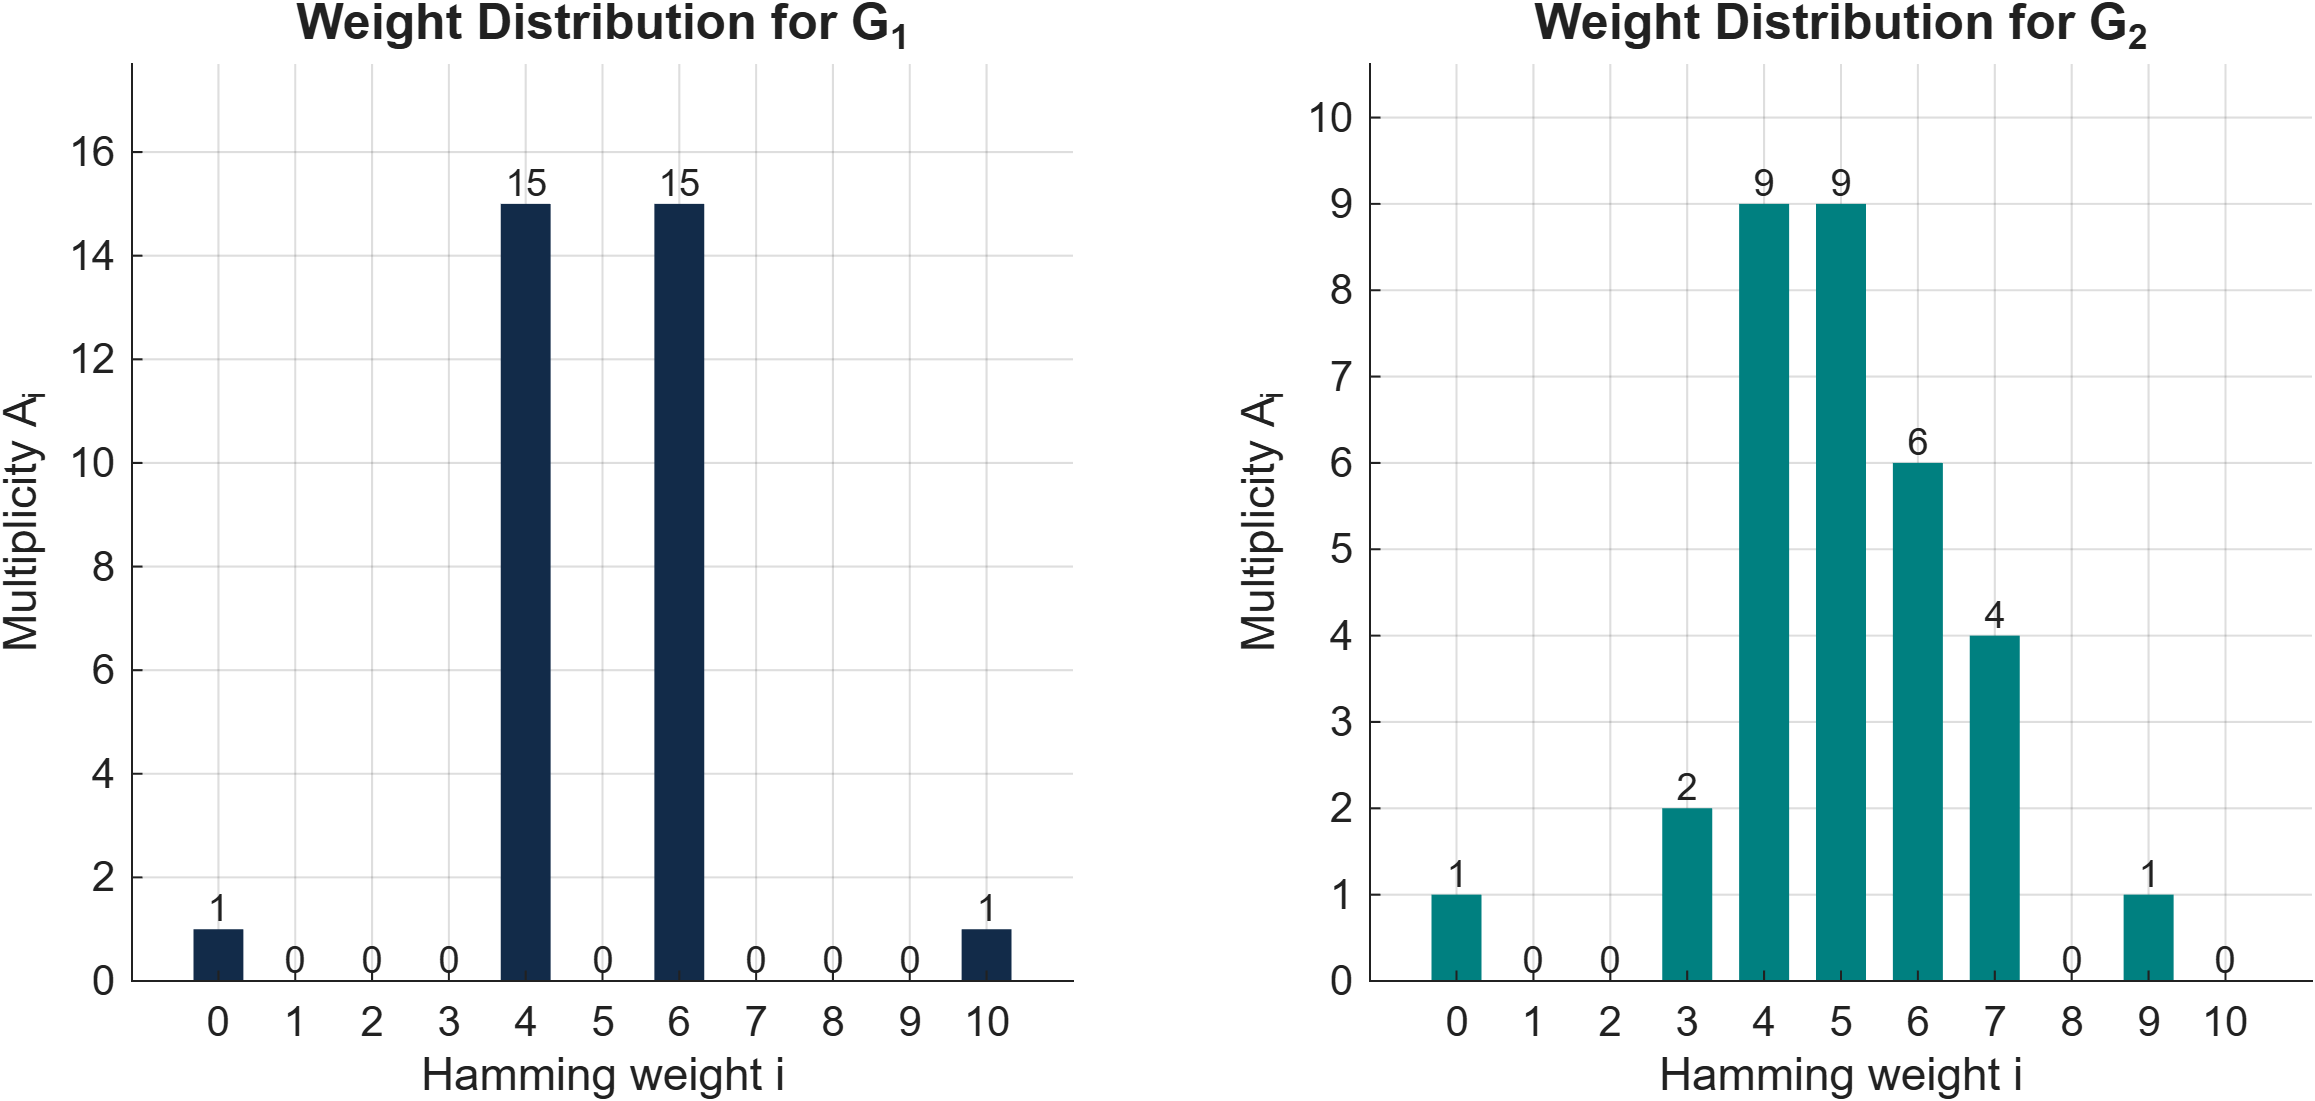
\includegraphics[width=\textwidth, height=4.0cm, keepaspectratio]{E1_P1_Q4.png}
		\end{column}
		
		% Tabella Code 1 (G1)
		\begin{column}{0.24\textwidth}
			\centering
			\scriptsize
			\renewcommand{\arraystretch}{0.82}
			\setlength{\tabcolsep}{4pt}
			\begin{tabular}{cc}
				\toprule
				\multicolumn{2}{c}{\textbf{Code 1 ($G_1$)}} \\
				\midrule
				\textbf{$i$} & \textbf{$A_i$} \\
				\midrule
				0  & 1  \\
				1  & 0  \\
				2  & 0  \\
				3  & 0  \\
				4  & 15 \\
				5  & 0  \\
				6  & 15 \\
				7  & 0  \\
				8  & 0  \\
				9  & 0  \\
				10 & 1  \\
				\bottomrule
			\end{tabular}
		\end{column}
		
		% Tabella Code 2 (G2)
		\begin{column}{0.24\textwidth}
			\centering
			\scriptsize
			\renewcommand{\arraystretch}{0.82}
			\setlength{\tabcolsep}{4pt}
			\begin{tabular}{cc}
				\toprule
				\multicolumn{2}{c}{\textbf{Code 2 ($G_2$)}} \\
				\midrule
				\textbf{$i$} & \textbf{$A_i$} \\
				\midrule
				0  & 1     \\
				1  & 0     \\
				2  & 0     \\
				3  & 2     \\
				4  & 9 	   \\
				5  & 9     \\
				6  & 6     \\
				7  & 4     \\
				8  & 0     \\
				9  & 1     \\
				10 & 0     \\
				\bottomrule
			\end{tabular}
		\end{column}
	\end{columns}
\end{frame}

% Slide 6
\begin{frame}{Exercise 1 - Part 1}
  \question{5. Determine the minimum $d_{\min}$ Hamming distance and its multiplicity $A_{\min}$.}

  \vspace{0.15cm}
  \begin{itemize}
    \item The minimum Hamming distance is the lowest distance possible from one codeword compared to all the others excluding the codewords at distance 0
    \item Since there are $2^k$ codewords the maximum multiplicity theoretically would be $32 - 1 = 31$ since the last vector is not computed due to the fact that the comparison would be redundant
    \item The first set of codewords reaches it since all the codewords have the same min distance
    \item While the second set has two different min distances with different multiplicities
  \end{itemize}

  \vspace{0.1cm}
  \centering
  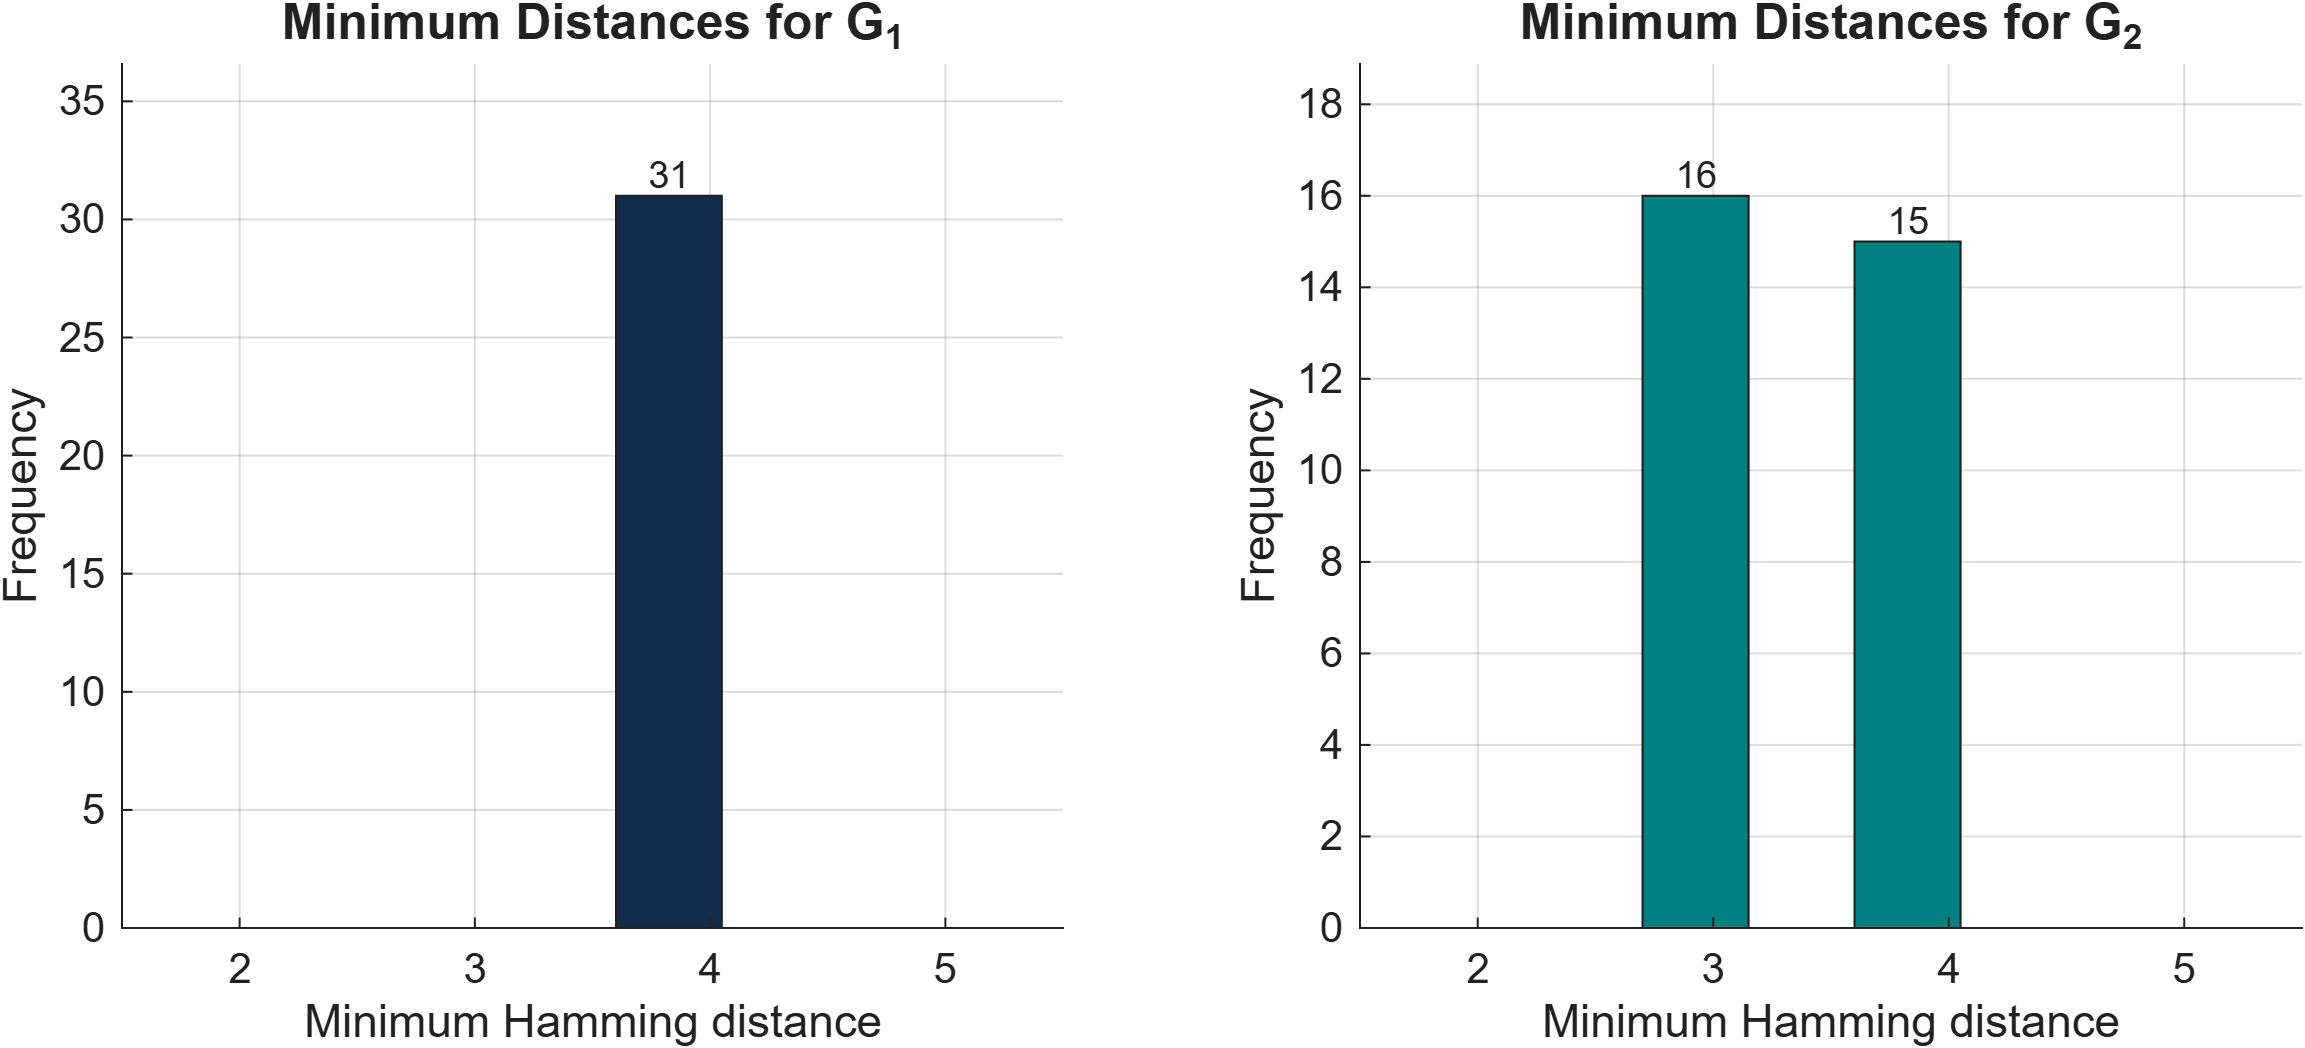
\includegraphics[width=0.88\textwidth, height=3.7cm, keepaspectratio]{E1_P1_Q5.png}
\end{frame}

% Slide 7
\begin{frame}[plain]
  \vfill
  \centering
  {\color{TealAccent}\rule{2cm}{2pt}}\\[0.4cm]
  {\LARGE\bfseries\color{NavyPrimary} Exercise 1 - Part 2}\\[0.2cm]
  {\large\color{SlateNeutral} Analytical Performance}
  \vfill
\end{frame}

% Slide 8
\begin{frame}{Exercise 1 - Part 2}
  \question{2. Plot both curves on the same log-log axes for $p \in [10^{-6}, 10^{-1}]$}

  \vspace{0.15cm}
  \begin{itemize}
    \item The plot shows 2 curves (with different generator matrix) of the probability of undetected error (PUE) ranging from a probability of $10^{-6}$ to $10^{-1}$
  \end{itemize}

  \vspace{0.1cm}
  \centering
  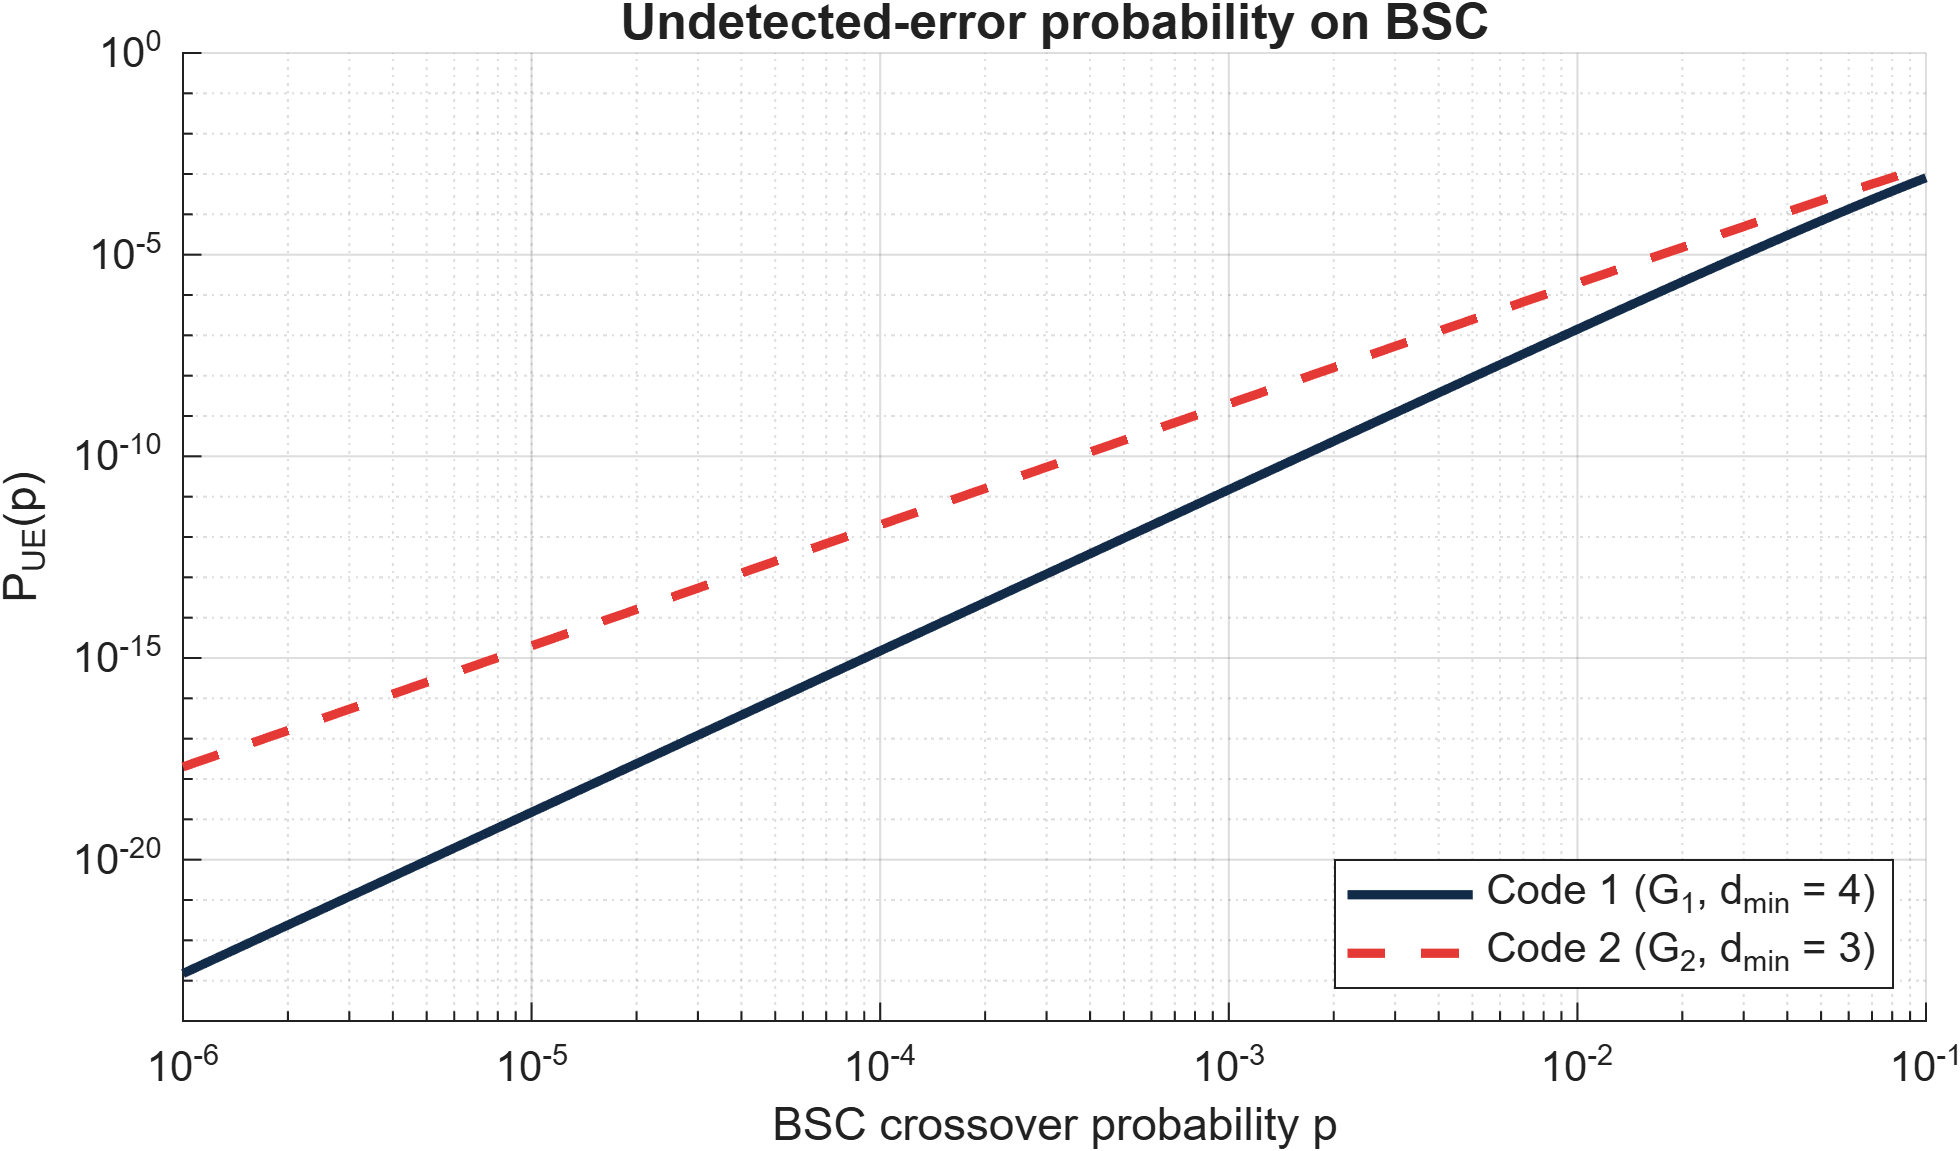
\includegraphics[width=0.78\textwidth, height=4.4cm, keepaspectratio]{E1_P2_Q2.png}
\end{frame}

% Slide 9
\begin{frame}{Exercise 1 - Part 2}
  \question{3. For small $p$, find the leading term of the two $P_{UE}$ expressions and explain its relationship with $d_{\min}$ and $A_{\min}$.}

  \vspace{0.3cm}
  \begin{itemize}
    \item For small probabilities, the '$(1-p)$' part of the sum can be discarded and the new formula contains only the multiplicity part multiplied by probability.
    \item For linear codes, the $d_{\min}$ between $c_1$ and $c_2$ is equivalent to the result of the XOR between the two codewords that is the Hamming weight.
  \end{itemize}
\end{frame}

% Slide 10
\begin{frame}{Exercise 1 - Part 2}
	\question{4. Compare the two codes: which one has better error-detection performance, and why?}
	
	\vspace{0.25cm}
	\begin{itemize}
		\item Code 1 is better because its curve lies below Code 2's curve, meaning that for a fixed bit error probability $p$, it achieves a lower $P_{UE}$.
		\item As you can see in the figure, Code 1 rather than Code 2 has a less rapid (steeper) curve that means better performance; for a logarithmic graph the $d_{\min}$ leads the gradient because $\log(A_{\min})$ is a constant.
		\item $\log(P_{UE}(p)) = \log(A_{\min}) + d_{\min} \cdot \log(p)$
		\item For small $p$ ($p \to 0$) the formula can be approximated to $P_{UE} \approx A_{d_{\min}} \cdot p^{d_{\min}}$, so:
		\begin{itemize}
			\item For $G_1$ the first non-null term is for $i = 4 \implies A_{\min} = 15 \implies$ the main term $P_{UE} \approx 15 p^4$
			\item For $G_2$ the first non-null term is for $i = 3 \implies A_{\min} = 2 \implies$ the main term $P_{UE} \approx 2 p^3$
		\end{itemize}
	\end{itemize}
\end{frame}

% Slide 11
\begin{frame}[plain]
  \vfill
  \centering
  {\color{TealAccent}\rule{2cm}{2pt}}\\[0.4cm]
  {\LARGE\bfseries\color{NavyPrimary} Exercise 1 - Part 3}\\[0.2cm]
  {\large\color{SlateNeutral} Syndrome Detector}
  \vfill
\end{frame}

% Slide 12
\begin{frame}{Exercise 1 - Part 3}
  \question{1. Construct the parity check matrix $H^T$ using the convention of the lectures:}
  \[
    H^T = \begin{bmatrix} P \\ I_5 \end{bmatrix}, \quad H^T \in \mathbb{F}_2^{10 \times 5}.
  \]
  {\small
  \renewcommand{\arraystretch}{0.9}
  \[
    H^T = \begin{bmatrix}
      1 & 1 & 1 & 0 & 0 \\
      0 & 1 & 1 & 1 & 0 \\
      0 & 0 & 1 & 1 & 1 \\
      1 & 0 & 0 & 1 & 1 \\
      1 & 1 & 0 & 0 & 1 \\
      \midrule
      1 & 0 & 0 & 0 & 0 \\
      0 & 1 & 0 & 0 & 0 \\
      0 & 0 & 1 & 0 & 0 \\
      0 & 0 & 0 & 1 & 0 \\
      0 & 0 & 0 & 0 & 1
    \end{bmatrix}
    \begin{array}{l}
      \left.\rule{0pt}{0.95cm}\right\} P \ (5 \times 5) \\[0.15cm]
      \left.\rule{0pt}{0.95cm}\right\} I_5 \ (5 \times 5)
    \end{array}
  \]
  }
\end{frame}

% Slide 13
\begin{frame}{Exercise 1 - Part 3}
  \question{2. Provide two received vectors $y_1$ and $y_2$ with zero and non-zero syndromes, respectively. Explain your choices.}

  \vspace{0.2cm}
  \begin{itemize}
    \item \textbf{Zero syndrome:}
    Encode message $m = 1\ 0\ 0\ 1\ 0$ directly via $y_1 = m \cdot G_1 \bmod 2$:
    \[
      y_1 = 1\ 0\ 0\ 1\ 0 \mid 0\ 1\ 1\ 1\ 1
    \]
    \[
      s_1 = y_1 \cdot H^T \bmod 2 = 0\ 0\ 0\ 0\ 0
    \]
    Because $y_1 \in C$ (no channel errors, $e = 0$).
    \item \textbf{Non-zero syndrome:}
    Single-bit error $e = \mathbf{1}\ 0\ 0\ 0\ 0\ 0\ 0\ 0\ 0\ 0$ into $y_1$:
    \[
      y_2 = y_1 \oplus e \bmod 2 = \mathbf{0}\ 0\ 0\ 1\ 0 \mid 0\ 1\ 1\ 1\ 1
    \]
    \[
      s_2 = y_2 \cdot H^T = e \cdot H^T \bmod 2 = 1\ 1\ 1\ 0\ 0
    \]
    Because $y_2 \notin C$, its syndrome equals the 1st row of $H^T$ ($1\ 1\ 1\ 0\ 0$).
  \end{itemize}
\end{frame}

% Slide 14
\begin{frame}{Exercise 1 - Part 3}
	\question{3. Construct a different matrix $H^T \in \mathbb{F}_2^{10 \times 5}$ such that a vector has zero syndrome if and only if it is a codeword. Compute the syndromes of the two vectors from Point 2.}
	
	\vspace{0.1cm}
	\begin{itemize}
		\item The equivalent Parity-Check Matrix $H_1^T$ is obtained with an elementary column operation over $\mathbb{F}_2$:
		{\small
			\[
			\begin{aligned}
				\text{New Col}_1 = \text{Col}_1 \oplus \text{Col}_2 &= [1\ 0\ 0\ 1\ 1\ 1\ 0\ 0\ 0\ 0]^T + [1\ 1\ 0\ 0\ 1\ 0\ 1\ 0\ 0\ 0]^T \\
				&= [\mathbf{0\ 1\ 0\ 1\ 0\ 1\ 1\ 0\ 0\ 0}]^T
			\end{aligned}
			\]
		}
		\item Adding two columns is an elementary operation that keeps the columns linearly independent and preserves the rank of $H^T$, so the vectors giving a zero syndrome remain the exact same codewords.
	\end{itemize}
	{\footnotesize
		\renewcommand{\arraystretch}{0.84}
		\[
		H_1^T = \begin{bmatrix}
			\mathbf{0} & 1 & 1 & 0 & 0 \\
			\mathbf{1} & 1 & 1 & 1 & 0 \\
			\mathbf{0} & 0 & 1 & 1 & 1 \\
			\mathbf{1} & 0 & 0 & 1 & 1 \\
			\mathbf{0} & 1 & 0 & 0 & 1 \\
			\mathbf{1} & 0 & 0 & 0 & 0 \\
			\mathbf{1} & 1 & 0 & 0 & 0 \\
			\mathbf{0} & 0 & 1 & 0 & 0 \\
			\mathbf{0} & 0 & 0 & 1 & 0 \\
			\mathbf{0} & 0 & 0 & 0 & 1
		\end{bmatrix}
		\]
	}
\end{frame}

% Slide 15
\begin{frame}{Exercise 1 - Part 3}
  \question{3. Construct a different matrix $H^T \in \mathbb{F}_2^{10 \times 5}$ such that a vector has zero syndrome if and only if it is a codeword. Compute the syndromes of the two vectors from Point 2.}

  \vspace{0.2cm}
  \begin{itemize}
    \item \textbf{Zero syndrome:}
    Encode message $m = 1\ 0\ 0\ 1\ 0$ directly via $y_1 = m \cdot G_1 \bmod 2$:
    \[
      y_1 = 1\ 0\ 0\ 1\ 0 \mid 0\ 1\ 1\ 1\ 1
    \]
    \[
      s_1' = y_1 \cdot H_1^T \bmod 2 = 0\ 0\ 0\ 0\ 0
    \]
    Because $y_1 \in C$ (no channel errors, $e = 0$).
    \item \textbf{Non-zero syndrome:}
    Single-bit error $e = \mathbf{1}\ 0\ 0\ 0\ 0\ 0\ 0\ 0\ 0\ 0$ into $y_1$:
    \[
      y_2 = y_1 \oplus e \bmod 2 = \mathbf{0}\ 0\ 0\ 1\ 0 \mid 0\ 1\ 1\ 1\ 1
    \]
    \[
      s_2' = y_2 \cdot H_1^T = e \cdot H_1^T \bmod 2 = 0\ 1\ 1\ 0\ 0
    \]
    Because $y_2 \notin C$, its syndrome equals the 1st row of $H_1^T$ ($0\ 1\ 1\ 0\ 0$).
  \end{itemize}
\end{frame}

% Slide 16
\begin{frame}{Exercise 1 - Part 3}
	\question{4. Construct a matrix $H^T \in \mathbb{F}_2^{10 \times 7}$ such that a vector has zero syndrome if and only if it is a codeword. Compute the syndromes of the two vectors from Point 2.}
	
	\vspace{0.1cm}
	\begin{itemize}
		\item The equivalent Parity-Check Matrix $H_2^T$ is obtained by appending two linearly dependent columns to $H^T$ by duplicating $\text{Col}_1$ and $\text{Col}_2$:
		\[
		H_2^T = \left[ H^T \mid \text{Col}_1(H^T)\ \text{Col}_2(H^T) \right]
		\]
		\item Since the two added columns are copies of the first two, they are linearly dependent on them: the rank remains $5$ (only redundant parity checks are added), so the vectors giving a zero syndrome remain the exact same codewords.
	\end{itemize}
	{\footnotesize
		\renewcommand{\arraystretch}{0.84}
		\[
		H_2^T = \begin{bmatrix}
			1 & 1 & 1 & 0 & 0 & \mathbf{1} & \mathbf{1} \\
			0 & 1 & 1 & 1 & 0 & \mathbf{0} & \mathbf{1} \\
			0 & 0 & 1 & 1 & 1 & \mathbf{0} & \mathbf{0} \\
			1 & 0 & 0 & 1 & 1 & \mathbf{1} & \mathbf{0} \\
			1 & 1 & 0 & 0 & 1 & \mathbf{1} & \mathbf{1} \\
			1 & 0 & 0 & 0 & 0 & \mathbf{1} & \mathbf{0} \\
			0 & 1 & 0 & 0 & 0 & \mathbf{0} & \mathbf{1} \\
			0 & 0 & 1 & 0 & 0 & \mathbf{0} & \mathbf{0} \\
			0 & 0 & 0 & 1 & 0 & \mathbf{0} & \mathbf{0} \\
			0 & 0 & 0 & 0 & 1 & \mathbf{0} & \mathbf{0}
		\end{bmatrix}
		\]
	}
\end{frame}

% Slide 17
\begin{frame}{Exercise 1 - Part 3}
  \question{4. Construct a matrix $H^T \in \mathbb{F}_2^{10 \times 7}$ such that a vector has zero syndrome if and only if it is a codeword. Compute the syndromes of the two vectors from Point 2.}

  \vspace{0.2cm}
  \begin{itemize}
    \item \textbf{Zero syndrome:}
    \[
      y_1 = 1\ 0\ 0\ 1\ 0 \mid 0\ 1\ 1\ 1\ 1
    \]
    \[
      s_1'' = y_1 \cdot H_2^T \bmod 2 = 0\ 0\ 0\ 0\ 0\ 0\ 0
    \]
    Because $y_1 \in C$ (no channel errors, $e = 0$).
    \item \textbf{Non-zero syndrome:}
    Single-bit error $e = \mathbf{1}\ 0\ 0\ 0\ 0\ 0\ 0\ 0\ 0\ 0$ into $y_1$:
    \[
      y_2 = y_1 \oplus e \bmod 2 = \mathbf{0}\ 0\ 0\ 1\ 0 \mid 0\ 1\ 1\ 1\ 1
    \]
    \[
      s_2'' = y_2 \cdot H_2^T = e \cdot H_2^T \bmod 2 = 1\ 1\ 1\ 0\ 0\ 1\ 1
    \]
    Because $y_2 \notin C$, its syndrome equals the 1st row of $H_2^T$ ($1\ 1\ 1\ 0\ 0\ 1\ 1$).
  \end{itemize}
\end{frame}

% Slide 18
\begin{frame}[plain]
  \vfill
  \centering
  {\color{TealAccent}\rule{2cm}{2pt}}\\[0.4cm]
  {\LARGE\bfseries\color{NavyPrimary} Exercise 1 - Part 4}\\[0.2cm]
  {\large\color{SlateNeutral} Monte Carlo Simulation}
  \vfill
\end{frame}

% Slide 19
\begin{frame}{Exercise 1 - Part 4}
  \question{1. Plot the two Monte Carlo curves (10 and 100 undetected errors) together with the analytical curve}

  \vspace{0.15cm}
  \centering
  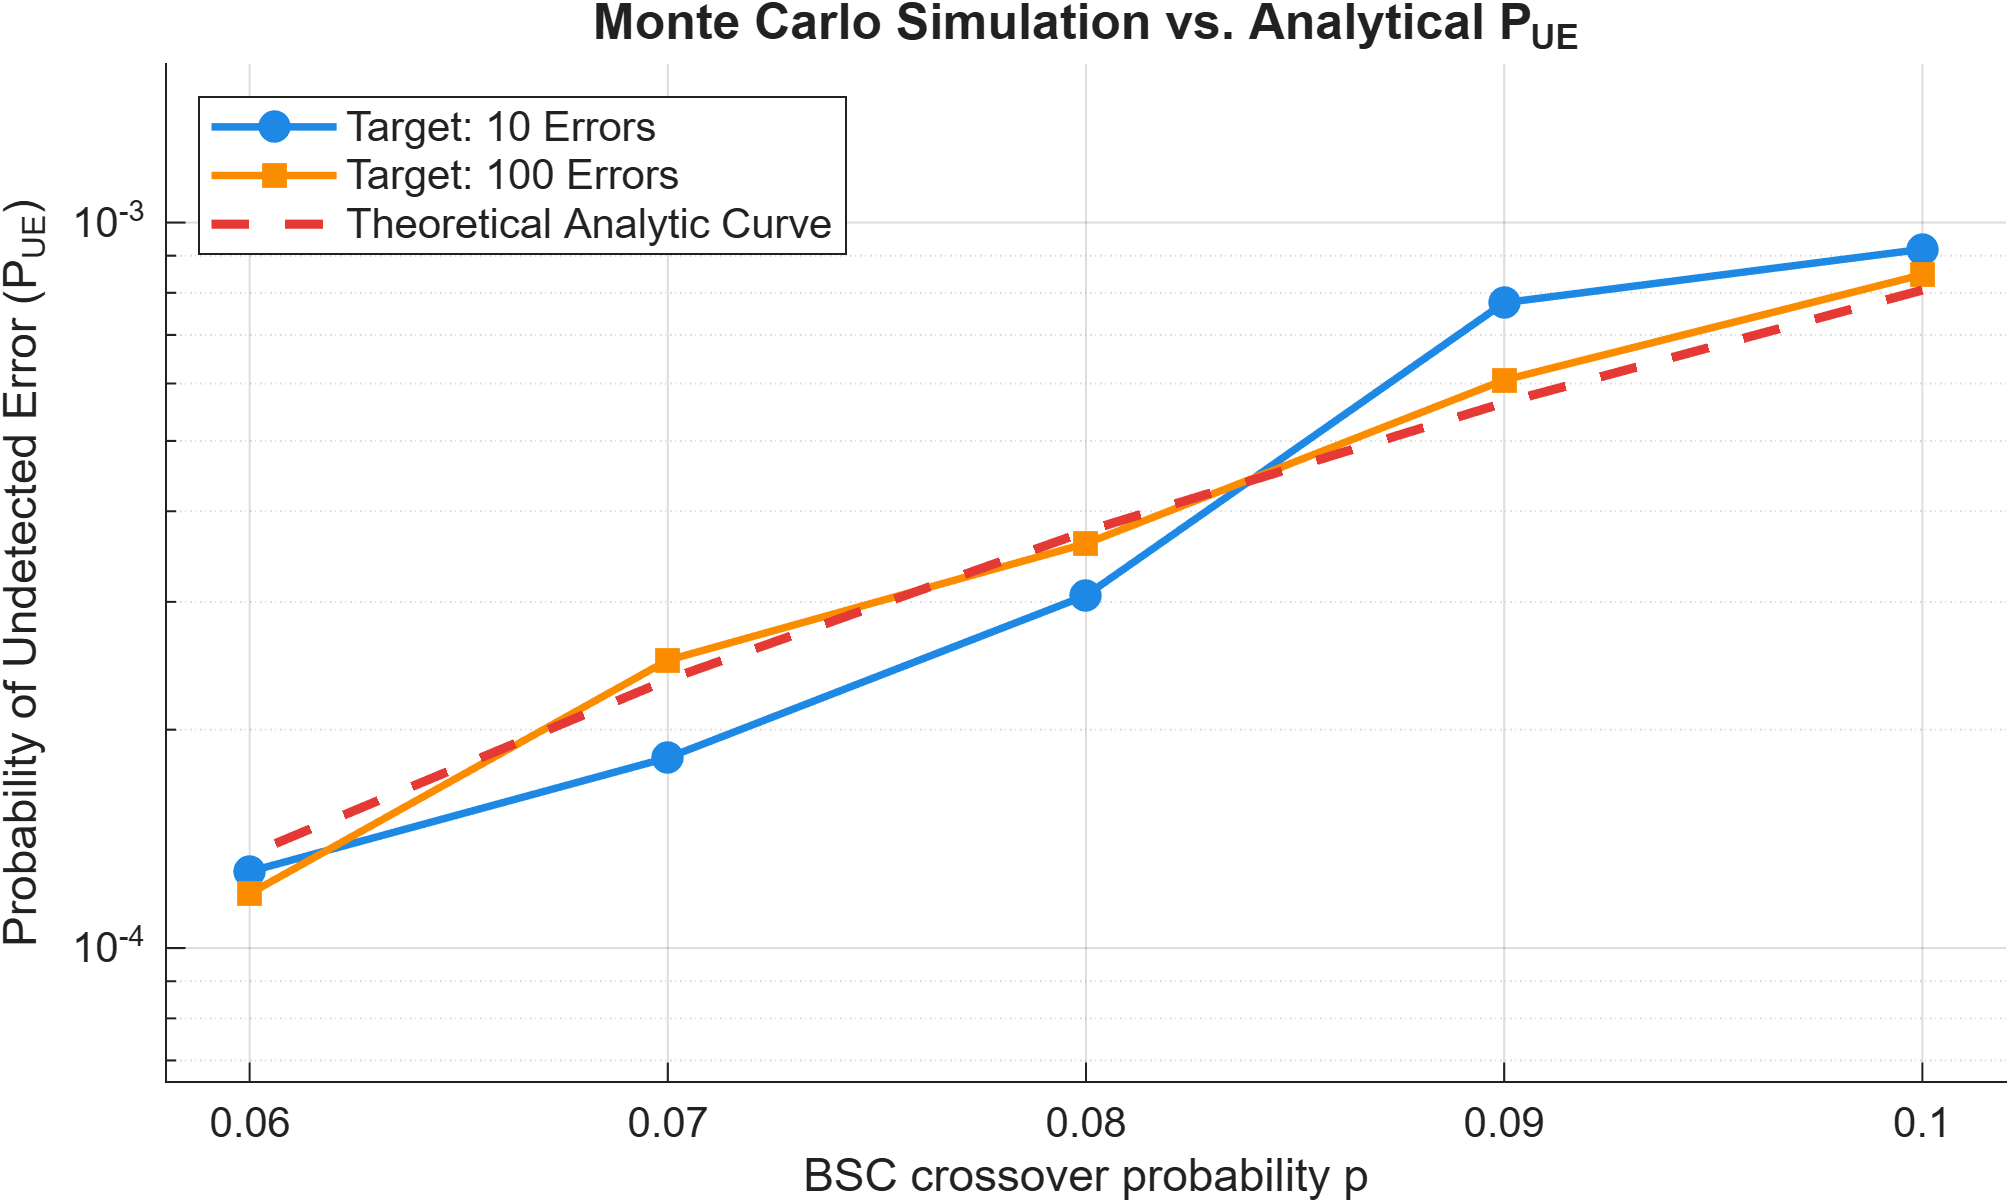
\includegraphics[width=0.82\textwidth, height=4.8cm, keepaspectratio]{E1_P4_Q1.png}
\end{frame}

% Slide 20
\begin{frame}{Exercise 1 - Part 4}
	\question{2. Explain what a confidence interval is and how it could be used to assess the reliability of the Monte Carlo estimates}
	
	\vspace{0.15cm}
	\begin{columns}[c]
		\begin{column}{0.55\textwidth}
			\footnotesize
			\begin{itemize}
				\item A confidence interval is an estimated range of values $[\hat{P}_{UE} - \Delta, \hat{P}_{UE} + \Delta]$, computed from a finite simulation sample, used to quantify the statistical uncertainty of a point estimate $\hat{P}_{UE}$.
				\item At a 95\% confidence level, repeating the simulation many times would produce intervals containing the true $P_{UE}$ in 95\% of runs.
				\item For rare events ($P_{UE} \ll 1$), the relative CI half-width depends strictly on the target error count $N_e$: $\Delta / P_{UE} \approx 1.96 / \sqrt{N_e}$.
				\item \textbf{Blue Curve ($N_e = 10$):} Relative uncertainty is $\pm 62\%$, explaining why the blue markers swing noticeably above ($p = 0.09$) and below ($p = 0.07$) the red dashed curve.
				\item \textbf{Orange Curve ($N_e = 100$):} Relative uncertainty drops to $\pm 19.6\%$ ($3.16\times$ tighter), keeping every orange point tightly aligned with the theoretical curve.
			\end{itemize}
		\end{column}
		\begin{column}{0.43\textwidth}
			\centering
			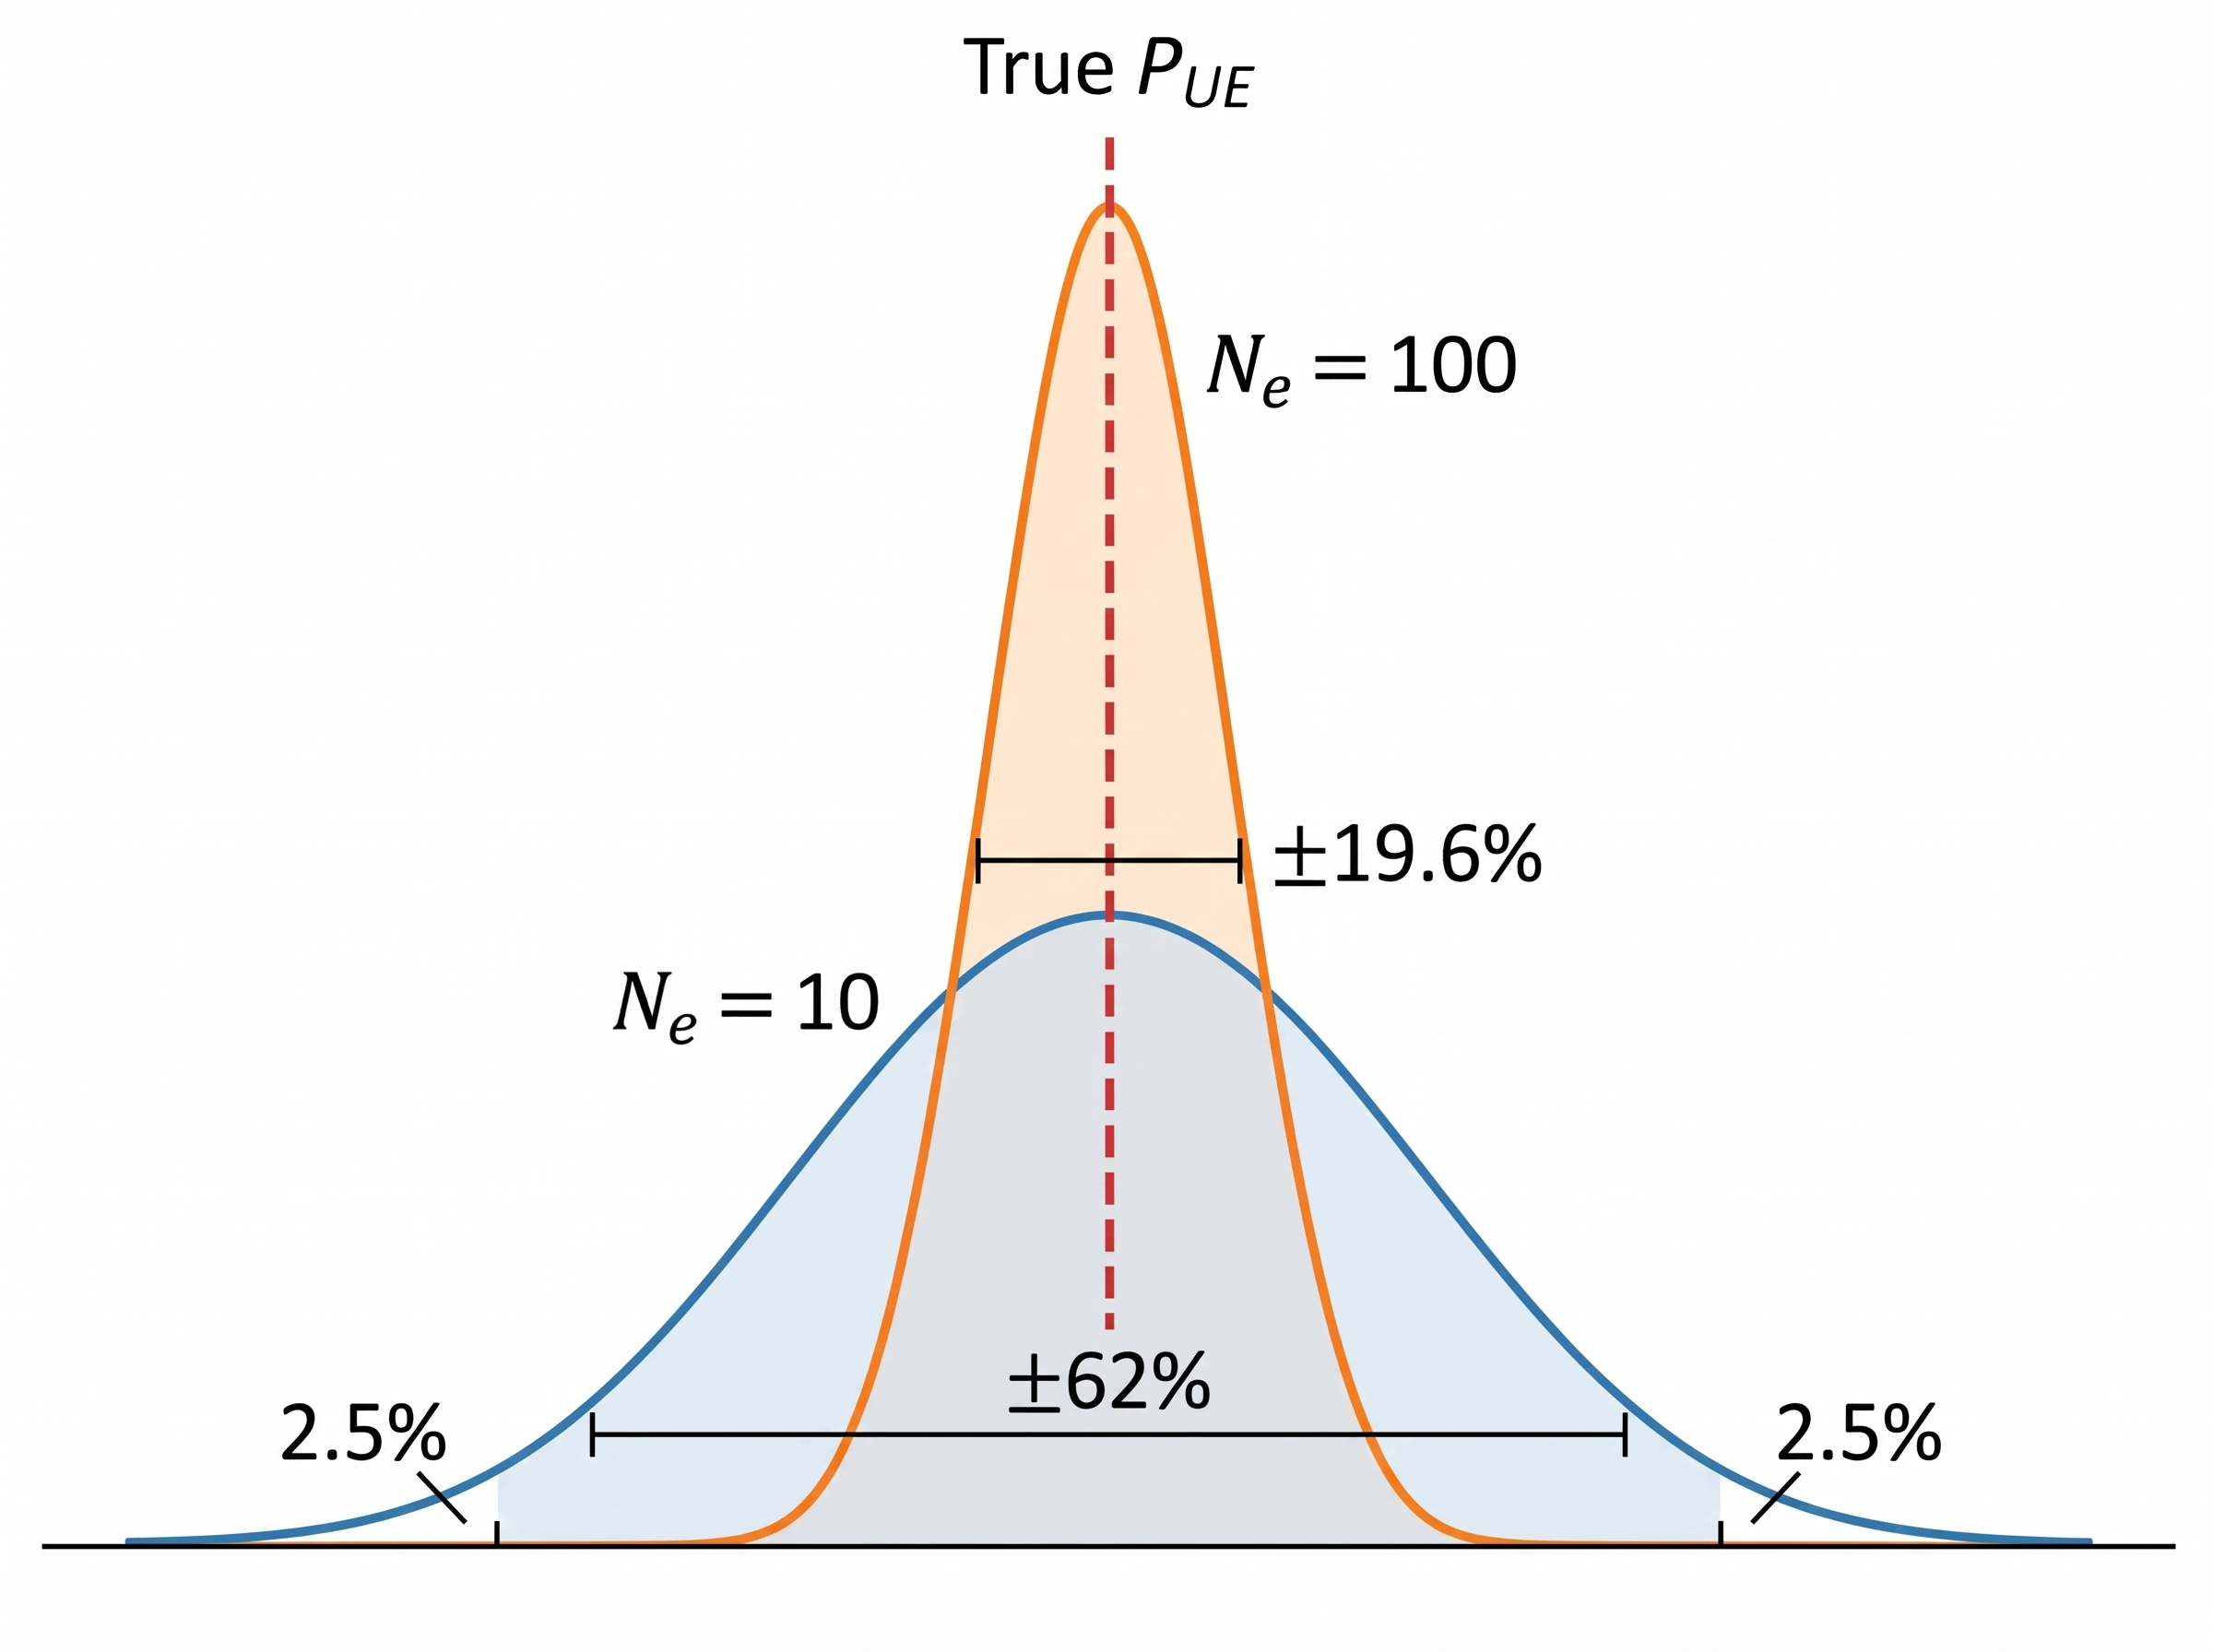
\includegraphics[width=\textwidth, height=4.4cm, keepaspectratio]{E1_P4_Q2.png}
		\end{column}
	\end{columns}
\end{frame}

% Slide 21
\begin{frame}{Exercise 1 - Part 4}
  \question{3. Compare the results, discussing statistical fluctuations, agreement with the analytical curve, and the trade-off between simulation accuracy and computational time.}

  \vspace{0.25cm}
  \begin{itemize}
    \item \textbf{Target 10 (Blue):} Shows significant random variance across $p \in [0.06, 0.10]$.
    \item \textbf{Target 100 (Orange):} Closely matches the Theoretical Analytic Curve across the entire range.
    \item Improving accuracy from 10 to 100 undetected errors requires $10\times$ more transmitted codewords.
    \item At $p = 0.06$ ($P_{UE} \approx 1.3 \times 10^{-4}$), collecting 100 undetected errors requires simulating roughly $7.7 \times 10^5$ codewords---showing how runtime grows inversely with $P_{UE}$ as $p$ decreases.
  \end{itemize}
\end{frame}

% Slide 22
\begin{frame}{Exercise 1 - Part 4}
	\question{3. Explain the advantages of having an analytical expression for $P_{UE}$.}
	
	\vspace{0.18cm}
	\begin{itemize}
		\item \textbf{Analytical Expression} ($n = 10$, $A_4 = 15$, $A_6 = 15$, $A_{10} = 1$):
		\[
		P_{UE} = \sum_{w=1}^{n} A_w \, p^w (1-p)^{n-w} = 15\,p^4(1-p)^6 + 15\,p^6(1-p)^4 + p^{10}
		\]
		\item The advantages are:
		\begin{itemize}
			\item Eliminates random Monte Carlo sampling noise, because it is a deterministic formula;
			\item Evaluates $P_{UE}$ in $n = 10$ operations for any $p$, whereas Monte Carlo runtime explodes as $1 / P_{UE}$ when $p \to 0$;
			\item Relates error-detection performance directly to the weight enumerator $A_w$ (multiplicity), enabling instant comparison across different linear codes.
		\end{itemize}
	\end{itemize}
\end{frame}

% Slide 23
\begin{frame}[plain]
  \vfill
  \centering
  {\color{TealAccent}\rule{2cm}{2pt}}\\[0.4cm]
  {\LARGE\bfseries\color{NavyPrimary} Exercise 1 - Part 5}\\[0.2cm]
  {\large\color{SlateNeutral} Retransmissions (ARQ)}
  \vfill
\end{frame}

% Slide 24
\begin{frame}{Exercise 1 - Part 5}
	\question{1. Write the expression of $p_0 = P_{\text{COR}, i=1}$, $p_1 = P_{\text{UE}, i=1}$, $p_2 = P_{\text{REJ}, i=1}$.}
	
	\vspace{0.15cm}
	\small
	\begin{itemize}
		\item \textbf{Correct Reception Probability} ($n = 10$):
		\[
		p_0 = P_{\text{COR}, i=1} = (1 - p)^n = (1 - p)^{10}
		\]
		\item \textbf{Undetected Error Probability} ($A_4 = 15$, $A_6 = 15$, $A_{10} = 1$):
		\[
		p_1 = P_{\text{UE}, i=1} = \sum_{w=1}^{n} A_w \, p^w (1 - p)^{n - w} = 15\,p^4(1-p)^6 + 15\,p^6(1-p)^4 + p^{10}
		\]
		\item \textbf{Block Rejection Probability}:
		\[
		\begin{aligned}
			p_2 = P_{\text{REJ}, i=1} &= 1 - p_0 - p_1 \\
			&= 1 - (1 - p)^{10} - \left[15\,p^4(1-p)^6 + 15\,p^6(1-p)^4 + p^{10}\right]
		\end{aligned}
		\]
	\end{itemize}
\end{frame}

% Slide 25
\begin{frame}{Exercise 1 - Part 5}
	\question{2. Write the analytical expression of $P_{\text{COR}, i}$ for $i = 1, 2, 3$.}
	
	\vspace{0.15cm}
	\small
	\begin{itemize}
		\item \textbf{1st Attempt ($i = 1$):}
		\[
		P_{\text{COR}, 1} = p_0 = (1 - p)^n = (1 - p)^{10}
		\]
		\item \textbf{2nd Attempt ($i = 2$):} (1 rejection followed by 1 correct reception)
		\[
		P_{\text{COR}, 2} = p_2 \cdot p_0 = (1 - p_0 - p_1) p_0 = \left[1 - (1-p)^{10} - p_1\right](1 - p)^{10}
		\]
		\item \textbf{3rd Attempt ($i = 3$):} (2 consecutive rejections followed by 1 correct reception)
		\[
		P_{\text{COR}, 3} = p_2^2 \cdot p_0 = (1 - p_0 - p_1)^2 p_0 = \left[1 - (1-p)^{10} - p_1\right]^2(1 - p)^{10}
		\]
	\end{itemize}
	{\footnotesize \textit{where $p_1 = 15\,p^4(1-p)^6 + 15\,p^6(1-p)^4 + p^{10}$.}}
\end{frame}

% Slide 26
\begin{frame}{Exercise 1 - Part 5}
  \question{3. Plot $1 - P(\text{COR}, i)$ versus $p$ over $10^{-2} \le p \le 10^{-1}$ for $i = 1, 2, 3$ on the same figure}

  \vspace{0.15cm}
  \centering
  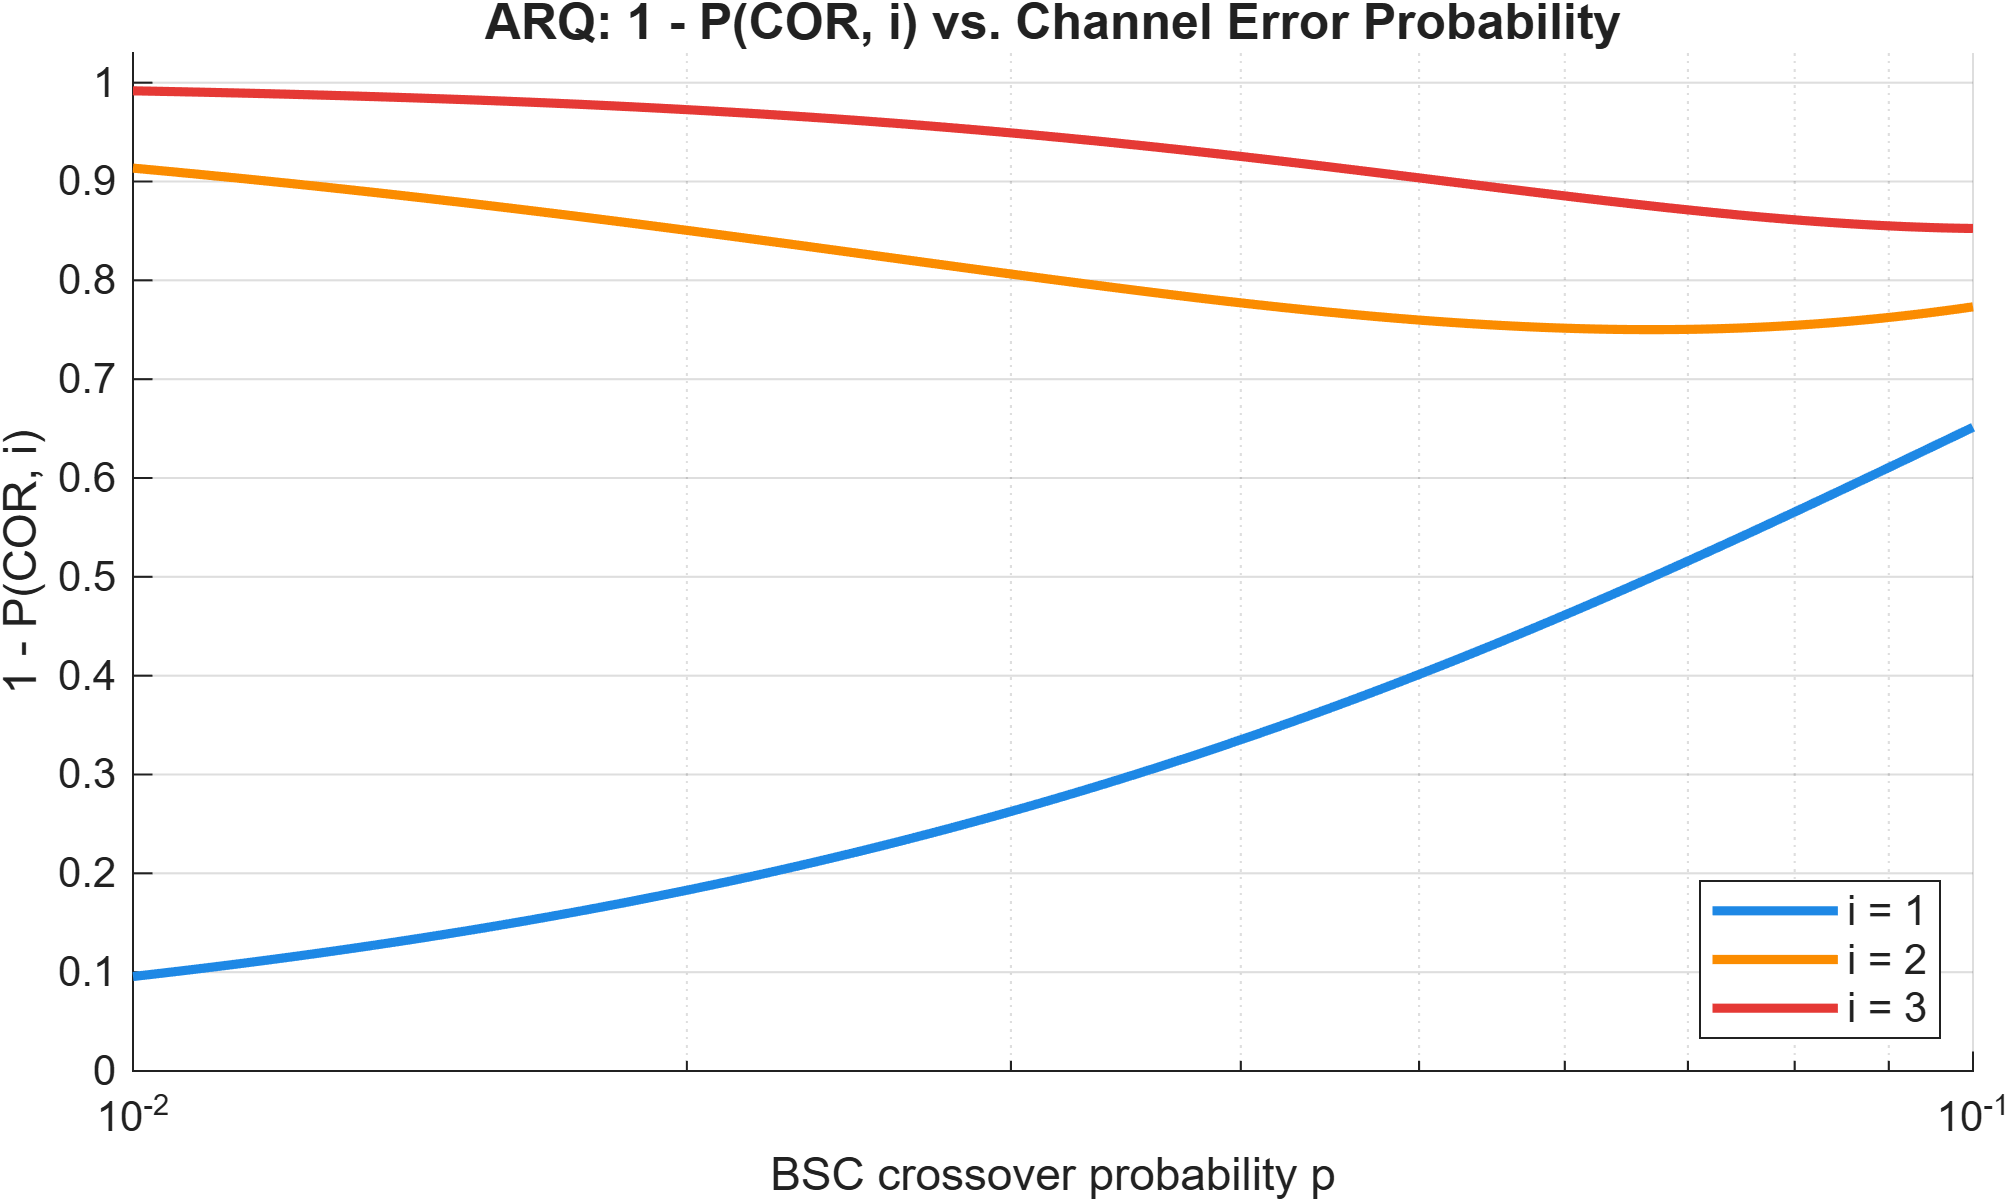
\includegraphics[width=0.82\textwidth, height=4.8cm, keepaspectratio]{E1_P5_Q3.png}
\end{frame}

% Slides 27-32: Exercise 1 - Part 6 (Discussion on ARQ)
\begin{frame}[plain]
  \vfill
  \centering
  {\color{TealAccent}\rule{2cm}{2pt}}\\[0.4cm]
  {\LARGE\bfseries\color{NavyPrimary} Exercise 1 - Part 6}\\[0.2cm]
  {\large\color{SlateNeutral} Discussion on ARQ}
  \vfill
\end{frame}

% Slide 28
\begin{frame}{Exercise 1 - Part 6}
	\question{1. Explain if allowing more transmission attempts increases the probability of correct reception}
	
	\vspace{0.25cm}
	\begin{itemize}
		\item \textbf{Yes:} Allowing more attempts $i$ increases the total probability of correct reception $P(\text{COR}, i)$:
		\[
		P(\text{COR}, i) = \sum_{k=1}^{i} p_2^{k-1} p_0 = p_0 \frac{1 - p_2^i}{1 - p_2}
		\]
		\item Whenever a block is rejected (with probability $p_2 < 1$), the transmitter gets another chance to send it correctly, adding a positive term $p_2^i p_0 > 0$.
		\item As $i$ grows, $P(\text{COR}, i)$ approaches its maximum limit $\frac{p_0}{p_0 + p_1}$ (meaning the failure curve $1 - P(\text{COR}, i)$ shifts downward, as seen in the previous plot).
	\end{itemize}
\end{frame}

% Slide 29
\begin{frame}{Exercise 1 - Part 6}
	\question{2. Explain if retransmissions can eliminate undetected errors.}
	
	\vspace{0.25cm}
	\begin{itemize}
		\item \textbf{No:} Retransmissions cannot eliminate undetected errors.
		\item ARQ only requests a retransmission when an error is detected ($s \neq 0$, probability $p_2$). If channel noise turns the sent codeword into another valid codeword ($s = 0$, probability $p_1$), the receiver accepts it and never asks for a retransmission.
		\item Allowing more attempts $i$ actually slightly increases the overall undetected error probability:
		\[
		P(\text{UE}, i) = p_1 \sum_{k=0}^{i-1} p_2^k = p_1 \frac{1 - p_2^i}{1 - p_2} \xrightarrow{i \to \infty} \frac{p_1}{p_0 + p_1}
		\]
	\end{itemize}
\end{frame}

% Slide 30
\begin{frame}{Exercise 1 - Part 6}
	\question{3. Discuss the trade-off between reliability and delay.}
	
	\vspace{0.25cm}
	\begin{itemize}
		\item Allowing more transmission attempts $i$ improves reliability: $P(\text{COR}, i)$ increases and the probability of dropping a packet after $i$ failed attempts ($p_2^i$) decreases.
		\item However, each retransmission adds extra delay (waiting for feedback and re-sending the block) and lowers the effective throughput because the channel is used multiple times for the same message.
		\item Small $i$: low latency and fast delivery, but higher packet loss when the channel is noisy.
		\item Large $i$: high reliability (up to the undetected error floor), at the cost of higher average and worst-case delay, especially at high $p$.
	\end{itemize}
\end{frame}

% Slide 31
\begin{frame}{Exercise 1 - Part 6}
	\question{4. Compute the expected number of transmissions for a maximum of $i = 1, 2, 3$ attempts, and generalize the result to an arbitrary $i$. (Hint: determine the probabilities of performing exactly 1, 2, or 3 transmissions, as applicable, and use them to compute the expected value.) What happens as $i \to \infty$? Discuss the result.}
	
	\vspace{0.1cm}
	\footnotesize
	\begin{itemize}
		\item A block is accepted with probability $1 - p_2 = p_0 + p_1$ and rejected (triggering a retransmission) with probability $p_2$:
		\begin{itemize}
			\item $i = 1$: $P(N = 1) = 1 \implies E[N]_1 = 1$
			\item $i = 2$: $P(N = 1) = 1 - p_2,\; P(N = 2) = p_2 \implies E[N]_2 = 1(1 - p_2) + 2p_2 = 1 + p_2$
			\item $i = 3$: $P(N = 1) = 1 - p_2,\; P(N = 2) = p_2(1 - p_2),\; P(N = 3) = p_2^2 \implies E[N]_3 = 1 + p_2 + p_2^2$
		\end{itemize}
		\item Generalizing for an arbitrary maximum number of attempts $i$:
		\[
		E[N]_i = \sum_{k=0}^{i-1} p_2^k = \frac{1 - p_2^i}{1 - p_2}
		\]
		\item As $i \to \infty$, since $0 \le p_2 < 1$, $p_2^i \to 0$ and the expected number of transmissions converges to a finite value:
		\[
		\lim_{i \to \infty} E[N]_i = \frac{1}{1 - p_2} = \frac{1}{p_0 + p_1}
		\]
		Even with unlimited attempts, the average delay remains finite (close to $1$ for small $p$) because rejections become geometrically unlikely.
	\end{itemize}
\end{frame}

% Slide 32
\begin{frame}{Exercise 1 - Part 6}
	\question{5. Use your result from Question 4 to support your discussion in Question 3.}
	
	\vspace{0.2cm}
	\footnotesize
	\begin{itemize}
		\item The expected number of transmissions $E[N]_i = \frac{1 - p_2^i}{1 - p_2}$ directly quantifies the average transmission delay and channel usage, while $P(\text{COR}, i) = p_0 \frac{1 - p_2^i}{1 - p_2}$ quantifies reliability.
		\item Both quantities scale with the same factor $\frac{1 - p_2^i}{1 - p_2}$: increasing $i$ reduces packet loss ($p_2^i$) and raises reliability, at the price of a higher average number of transmissions $E[N]_i$ (lower throughput and higher latency).
		\item At low $p$ ($p_2 \ll 1$), higher-order terms $p_2^k$ vanish rapidly, so $E[N]_i \approx 1$ even for large $i$: we gain reliability with almost zero extra average delay.
		\item At high $p$ ($p_2$ closer to $1$), increasing $i$ significantly boosts $E[N]_i$ toward $\frac{1}{1 - p_2}$, making the latency penalty substantial.
	\end{itemize}
\end{frame}

% ==============================================================================
% EXERCISE 2a & 2b: CRC (Slides 33-48)
% ==============================================================================
\begin{frame}[plain]
  \vfill
  \centering
  {\color{TealAccent}\rule{2cm}{2pt}}\\[0.4cm]
  {\LARGE\bfseries\color{NavyPrimary} Exercise 2a}\\[0.2cm]
  {\large\color{SlateNeutral} CRC Codes and Weight Distribution}
  \vfill
\end{frame}

\begin{frame}{Exercise 2a}
  \question{1. Choose a primitive binary polynomial $p(D)$ of degree $r$.}

  \vspace{0.3cm}
  \begin{itemize}
    \item For this part, we selected the primitive binary polynomial of degree $r_p = 3$:
    \[
      p(D) = D^3 + D + 1
    \]
  \end{itemize}
\end{frame}

\begin{frame}{Exercise 2a}
  \question{2. Construct the generator polynomial $g(D) = (D+1)p(D)$.}

  \vspace{0.3cm}
  \begin{itemize}
    \item The generator polynomial $g(D)$ is obtained by multiplying the primitive polynomial $p(D)$ by $(D+1)$:
    \[
      g(D) = (D+1)p(D) = (D+1)(D^3 + D + 1) = D^4 + D^3 + D^2 + 1
    \]
  \end{itemize}
\end{frame}

\begin{frame}{Exercise 2a}
  \question{5. Construct a table containing the four information vectors $v$, the corresponding information polynomials $v(D)$, the codeword polynomials $c(D)$, the codeword vectors $c$, and their Hamming weights.}

  \vspace{0.5cm}
  \centering
  \footnotesize
  \setlength{\tabcolsep}{4.5pt}
  \begin{tabular}{ccccc}
    \toprule
    \textbf{Information} & \textbf{Information} & \textbf{Codeword} & \textbf{Codeword} & \textbf{Hamming} \\
    \textbf{vectors $v$} & \textbf{polynomials $v(D)$} & \textbf{polynomials $c(D)$} & \textbf{vectors $c$} & \textbf{weight $w_H$} \\
    \midrule
    $0\ 0$ & $0$ & $0$ & $0\ 0\ 0\ 0\ 0\ 0$ & $0$ \\
    $0\ 1$ & $1$ & $D^4 + D^3 + D^2 + 1$ & $0\ 1\ 1\ 1\ 0\ 1$ & $4$ \\
    $1\ 0$ & $D$ & $D^5 + D^2 + D + 1$ & $1\ 0\ 0\ 1\ 1\ 1$ & $4$ \\
    $1\ 1$ & $D+1$ & $D^5 + D^4 + D^3 + D$ & $1\ 1\ 1\ 0\ 1\ 0$ & $4$ \\
    \bottomrule
  \end{tabular}
\end{frame}

\begin{frame}{Exercise 2a}
  \question{6. Compute the weight distribution coefficients $A_i$}

  \vspace{0.25cm}
  \begin{columns}[T]
    \begin{column}{0.35\textwidth}
      \centering
      \small
      \begin{tabular}{c}
        \toprule
        \textbf{Weight coefficients $A_i$} \\
        \midrule
        $A_0 = 1$ \\
        $A_1 = 0$ \\
        $A_2 = 0$ \\
        $A_3 = 0$ \\
        $A_4 = 3$ \\
        $A_5 = 0$ \\
        $A_6 = 0$ \\
        \bottomrule
      \end{tabular}
    \end{column}
    \begin{column}{0.62\textwidth}
      \vspace{0.3cm}
      \begin{itemize}
        \item The weight distribution shows that the code contains one codeword of weight 0 and three codewords of weight 4.
        \item All other weight values have a zero coefficient.
      \end{itemize}
    \end{column}
  \end{columns}
\end{frame}

\begin{frame}{Exercise 2a}
  \question{7. Comment on the results}

  \vspace{0.25cm}
  \begin{itemize}
    \item The code has a minimum Hamming distance of $d_{\min} = 4$, which guarantees the detection of up to 3 bit errors and the correction of a single-bit error.
    \item Another important property is that all codewords have an even Hamming weight ($w_H \in \{0, 4, 6\}$). This is ensured by the presence of the factor $(D+1)$ in the generator polynomial, which forces every codeword to contain an even number of ones.
    \item As a result, the code can detect any channel error involving an odd number of bit flips, since such errors change the parity of the received word, making it immediately recognizable as an invalid codeword.
  \end{itemize}
\end{frame}

\begin{frame}{Exercise 2a}
  \question{9. Present a table reporting the weight distribution coefficients $A_i$ for each value of $k$ considered}

  \vspace{0.25cm}
  \centering
  \small
  \renewcommand{\arraystretch}{0.92}
  \begin{tabular}{ccc}
    \toprule
    $\mathbf{k = 2 \quad (n = 6)}$ & $\mathbf{k = 3 \quad (n = 7)}$ & $\mathbf{k = 4 \quad (n = 8)}$ \\
    \midrule
    $A_0 = 1$ & $A_0 = 1$ & $A_0 = 1$ \\
    $A_1 = 0$ & $A_1 = 0$ & $A_1 = 0$ \\
    $A_2 = 0$ & $A_2 = 0$ & $A_2 = 1$ \\
    $A_3 = 0$ & $A_3 = 0$ & $A_3 = 0$ \\
    $A_4 = 3$ & $A_4 = 7$ & $A_4 = 11$ \\
    $A_5 = 0$ & $A_5 = 0$ & $A_5 = 0$ \\
    $A_6 = 0$ & $A_6 = 0$ & $A_6 = 3$ \\
    --- & $A_7 = 0$ & $A_7 = 0$ \\
    --- & --- & $A_8 = 0$ \\
    \bottomrule
  \end{tabular}
\end{frame}

\begin{frame}{Exercise 2a}
  \question{10. Explain mathematically why weight-2 codewords appear for exactly that value of $k$.}

  \vspace{0.15cm}
  \small
  \begin{itemize}
    \item A codeword with Hamming weight 2 can be expressed as: $c(D) = D^i + D^j = D^j(D^L + 1)$ where $L = i - j$ is the distance between the two non-zero bits.
    \item Since a valid codeword must be divisible by the generator polynomial $g(D) = (D+1)p(D)$, with $p(D) = D^3 + D + 1$, the polynomial $p(D)$ must divide $D^L + 1$.
    \item Being a primitive polynomial of degree 3, $p(D)$ has order: $N = 2^3 - 1 = 7$.
    \item Therefore, the smallest possible distance is $L = 7$. The corresponding minimum codeword is: $c(D) = D^7 + 1$.
    \item Its degree is 7, requiring a codeword length of at least $n = 8$. Since $n = k + r$, with $r = 4$: $k + 4 \ge 8 \implies k \ge 4$.
    \item \textbf{Conclusion:} Weight-2 codewords first appear at $k = 4$, because this is the minimum information length that allows two non-zero bits separated by 7 positions.
  \end{itemize}
\end{frame}

% Exercise 2b
\begin{frame}[plain]
  \vfill
  \centering
  {\color{TealAccent}\rule{2cm}{2pt}}\\[0.4cm]
  {\LARGE\bfseries\color{NavyPrimary} Exercise 2b}\\[0.2cm]
  {\large\color{SlateNeutral} CRC Codes -- Burst Error Detection}
  \vfill
\end{frame}

\begin{frame}{Exercise 2b}
  \question{1. What is the maximum burst length $L$ that is certainly detected by this CRC code?}

  \vspace{0.25cm}
  \begin{itemize}
    \item A CRC code with $r$ redundancy bits guarantees the detection of all burst errors of length:
    \[
      L \le r
    \]
    \item Since the generator polynomial has degree $r = 4$, the code is guaranteed to detect all burst errors of length up to:
    \[
      L_{\max} = 4\text{ bits}
    \]
    \item Therefore, this CRC code detects with certainty any burst error of length 4 bits or less.
  \end{itemize}
\end{frame}

\begin{frame}{Exercise 2b}
  \question{2. Provide a mathematical proof of your answers using the polynomial representation of burst errors}

  \vspace{0.15cm}
  \small
  \begin{itemize}
    \item A burst error of length $L$ can be represented as $e(D) = D^j b(D)$, where $b(D)$ is the burst polynomial with degree $\deg b(D) = L - 1$, and $D^j$ represents the position of the burst within the transmitted block.
    \item An error goes undetected if and only if it is divisible by the generator polynomial $g(D)$. Since $g(0) = 1$, $D^j$ and $g(D)$ are relatively prime. Therefore:
    \[
      g(D) \mid e(D) \iff g(D) \mid b(D)
    \]
    \item For burst lengths $L \le r$, we have:
    \[
      \deg b(D) = L - 1 \le r - 1 < r = \deg g(D)
    \]
    \item Thus, $b(D)$ cannot be a non-zero multiple of $g(D)$. Every burst error of length $L \le r = 4$ is guaranteed to be detected by the CRC code.
  \end{itemize}
\end{frame}

\begin{frame}{Exercise 2b}
  \question{3. Find two burst error patterns $e_1$ and $e_2$}

  \vspace{0.25cm}
  \begin{itemize}
    \item \textbf{1. Detected burst error ($L = 4$):}
    \[
      e_1 = [1\ 0\ 1\ 1\ 0\ 0\ 0\ 0]^T
    \]
    Its polynomial representation is:
    \[
      e_1(D) = D^3 + D + 1
    \]
    \item \textbf{2. Undetected burst error ($L = 5$):}
    \[
      e_2 = [1\ 1\ 1\ 0\ 1\ 0\ 0\ 0]^T
    \]
    Its polynomial representation is:
    \[
      e_2(D) = D^4 + D^3 + D^2 + 1 = g(D)
    \]
  \end{itemize}
\end{frame}

\begin{frame}{Exercise 2b}
  \question{4. Explain mathematically why one error is detected and the other is not}

  \vspace{0.2cm}
  \small
  \begin{itemize}
    \item The first error polynomial is $e_1(D) = D^3 + D + 1$. Since its degree is smaller than the degree of the generator polynomial ($\deg e_1 = 3 < \deg g = 4$), it cannot be divisible by $g(D)$.
    \item Therefore, the division produces a non-zero remainder:
    \[
      \text{rem}\left(\frac{e_1(D)}{g(D)}\right) = D^3 + D + 1 \ne 0
    \]
    The syndrome is non-zero, so the CRC detects the error.
    \item The second error polynomial is $e_2(D) = D^4 + D^3 + D^2 + 1 = g(D)$. Since the error polynomial coincides with the generator polynomial, the division gives:
    \[
      \text{rem}\left(\frac{e_2(D)}{g(D)}\right) = 0
    \]
    The syndrome is zero, meaning that the error is indistinguishable from a valid codeword.
  \end{itemize}
\end{frame}

\begin{frame}{Exercise 2b}
  \question{5. Choose a codeword and verify your results}

  \vspace{0.25cm}
  \begin{itemize}
    \item The selected information sequence is:
    \[
      v = [1\ 0\ 1\ 1]^T
    \]
    \item Using the CRC encoder with generator polynomial $g(D) = D^4 + D^3 + D^2 + 1$, the resulting codeword is:
    \[
      c = [1\ 0\ 1\ 1\ 0\ 0\ 1\ 0]^T
    \]
    \item Two transmission scenarios were tested:
    \begin{itemize}
      \item \textbf{Burst error ($e_1$), $L = 4$:} detected by the CRC (non-zero syndrome).
      \item \textbf{Burst error ($e_2$), $L = 5$:} not detected by the CRC (zero syndrome).
    \end{itemize}
  \end{itemize}
\end{frame}

% ==============================================================================
% EXERCISE 3a, 3b, 3c: Decision Regions
% ==============================================================================
\begin{frame}[plain]
  \vfill
  \centering
  {\color{TealAccent}\rule{2cm}{2pt}}\\[0.4cm]
  {\LARGE\bfseries\color{NavyPrimary} Exercise 3a}\\[0.2cm]
  {\large\color{SlateNeutral} Decision Regions property for a linear code}
  \vfill
\end{frame}

% --- Slide 1/2 ---
\begin{frame}{Exercise 3a}
  \question{1. Prove that, for every codeword $c \in C$, $D(c) = c + D(0)$ (1/2).}

  \vspace{0.1cm}
  \begin{itemize}
    \item Consider a binary linear code $C(n,k)$ with minimum-distance decoding. Writing $y = c + e$ (so $y + c = e$) and $c' = c + c''$ (so $c' + c = c'' \in C$ since $C$ is linear), we develop $D(c)$ in four steps:
    \[
      \begin{aligned}
        D(c) &= \{ y \in \mathbb{F}_2^n : d_H(y, c) \le d_H(y, c'), \; \forall c' \in C \} \\
             &= \{ c + e \in \mathbb{F}_2^n : d_H(c + e + c, c + c) \le d_H(c + e + c, c' + c), \; \forall c' \in C \} \\
             &= \{ c + e \in \mathbb{F}_2^n : d_H(e, 0) \le d_H(e, c''), \; \forall c'' \in C \} \\
             &= \{ c + e \in \mathbb{F}_2^n : w_H(e) \le d_H(e, c''), \; \forall c'' \in C \}
      \end{aligned}
    \]
  \end{itemize}
\end{frame}

% --- Slide 2/2 ---
\begin{frame}{Exercise 3a}
  \question{1. Prove that, for every codeword $c \in C$, $D(c) = c + D(0)$ (2/2).}

  \vspace{0.08cm}
  \begin{itemize}
    \item Similarly, developing $D(0)$ with $y = c + e$ and $d_H(y, 0) = w_H(y)$:
    \[
      \begin{aligned}
        D(0) &= \{ y \in \mathbb{F}_2^n : d_H(y, 0) \le d_H(y, c'), \; \forall c' \in C \} \\
             &= \{ c + e \in \mathbb{F}_2^n : w_H(c + e) \le d_H(c + e, c'), \; \forall c' \in C \} \\
             &\text{with } c = 0\text{, so} \\
             &= \{ 0 + e \in \mathbb{F}_2^n : w_H(0 + e) \le d_H(0 + e, c'), \; \forall c' \in C \} \\
             &= \{ e \in \mathbb{F}_2^n : w_H(e) \le d_H(e, c'), \; \forall c' \in C \}
      \end{aligned}
    \]
    \item Writing $D(0) = \{e_0, e_1, \dots, e_{N-1}\}$, since every element in $D(c)$ has the form $y = c + e$:
    \[
      D(c) = \{ c + e_0, c + e_1, \dots, c + e_{N-1} \} = \{ e_0, e_1, \dots, e_{N-1} \} + c = D(0) + c = c + D(0)
    \]
  \end{itemize}
\end{frame}

\begin{frame}{Exercise 3a}
  \question{2. Discuss the meaning of this property}

  \vspace{0.25cm}
  \begin{itemize}
    \item All decision regions $D(c)$ have the exact same shape and size, since each one is simply $D(0)$ shifted by the codeword $c$.
    \item Because every codeword has the exact same set of correctable error patterns around it, the word error probability $P_W(E)$ over a BSC does not depend on the transmitted codeword (so in analysis or simulations we can just assume the all-zero codeword $0$ was sent).
    \item Instead of storing $2^k$ separate decision regions, the decoder only needs to store $D(0)$ (the coset leaders) and subtract the error vector $e \in D(0)$ from the received word $y$.
  \end{itemize}
\end{frame}

\begin{frame}[plain]
  \vfill
  \centering
  {\color{TealAccent}\rule{2cm}{2pt}}\\[0.4cm]
  {\LARGE\bfseries\color{NavyPrimary} Exercise 3b}\\[0.2cm]
  {\large\color{SlateNeutral} Decision Regions of a linear code}
  \vfill
\end{frame}

\begin{frame}{Exercise 3b}
  \question{1. Choose a non-systematic generator matrix $G$ of rank 3.}

  \vspace{0.2cm}
  \begin{itemize}
    \item \textbf{Non-Systematic Generator Matrix $G$:}
    \[
      G = \begin{bmatrix}
        1 & 1 & 0 & 1 & 0 & 1 \\
        0 & 1 & 1 & 0 & 1 & 1 \\
        1 & 1 & 1 & 1 & 1 & 0
      \end{bmatrix}
    \]
    \item Dimensions: $3 \times 6$ ($k = 3$ information bits, $n = 6$ coded bits)
    \item Does not contain an identity submatrix $I_3$ so is in Non-systematic form.
  \end{itemize}
\end{frame}

\begin{frame}{Exercise 3b}
  \question{5. Write all the decision regions $D(c)$}

  \vspace{0.15cm}
  \footnotesize
  \begin{itemize}
    \item $D(c_1)$ : Codeword $\mathbf{000000}$: $\{\mathbf{000000}, 000001, 000010, 000100, 001000, 100000, 000110, 001100, 100010, 101000\}$
    \item $D(c_2)$ : Codeword $\mathbf{111110}$: $ \{\mathbf{111110}, 111111, 111100, 111010, 110110, 011110, 111000, 110010, 011100, 010110\}$
    \item $D(c_3)$ : Codeword $\mathbf{011011}$: $ \{\mathbf{011011}, 011010, 011001, 011111, 010011, 111011, 011101, 010111, 111001, 110011\}$
    \item $D(c_4)$ : Codeword $\mathbf{100101}$: $\{\mathbf{100101}, 100100, 100111, 100001, 101101, 000101, 100011, 101001, 000111, 001101\}$
    \item $D(c_5)$ : Codeword $\mathbf{110101}$: $\{\mathbf{110101}, 110100, 110111, 110001, 111101, 010101, 110011, 111001, 010111, 011101\}$
    \item $D(c_6)$ : Codeword $\mathbf{001011}$: $\{\mathbf{001011}, 001010, 001001, 001111, 000011, 101011, 001101, 000111, 101001, 100011\}$
    \item $D(c_7)$ : Codeword $\mathbf{101110}$: $\{\mathbf{101110}, 101111, 101100, 101010, 100110, 001110, 101000, 100010, 001100, 000110\}$
    \item $D(c_8)$ : Codeword $\mathbf{010000}$: $\{\mathbf{010000}, 010001, 010010, 010100, 011000, 110000, 010110, 011100, 110010, 111000\}$
  \end{itemize}
\end{frame}

\begin{frame}{Exercise 3b}
  \question{5. Write all the decision regions $D(c)$}

  \vspace{0.25cm}
  \begin{itemize}
    \item Here, each region includes all vectors closest to $c_i$ without arbitrary tie-breaking:
    \begin{itemize}
      \item 1 vector at $d_H = 0$ (the codeword itself)
      \item 6 vectors at $d_H = 1$ (all single-bit errors, uniquely decoded since $d_{\min} = 3$)
      \item 3 vectors at $d_H = 2$ (boundary vectors equidistant from another codeword)
    \end{itemize}
    \item Overlapping regions ($8 \times 10 = 80 > 64$), where 24 boundary vectors appear in multiple regions (3 per codeword).
  \end{itemize}
\end{frame}

\begin{frame}{Exercise 3b}
  \question{6. Verify that $D(c) = c + D(0), \quad \forall c \in C$}

  \vspace{0.25cm}
  \begin{itemize}
    \item Verification Logic implemented in MATLAB:
    \begin{itemize}
      \item Extract the reference region $D_0$ corresponding to $c_1 = 0\ 0\ 0\ 0\ 0\ 0$
      \item Compute the shifted set $D_C = c_i \oplus D_0 \bmod 2$
      \item Compare sorted sets with the command: \texttt{isequal(sortrows(y\_region), sortrows(D\_C))} $\rightarrow$ Rule Verified for all $i \in \{1, \dots, 8\}$
    \end{itemize}
  \end{itemize}
\end{frame}

\begin{frame}[plain]
  \vfill
  \centering
  {\color{TealAccent}\rule{2cm}{2pt}}\\[0.4cm]
  {\LARGE\bfseries\color{NavyPrimary} Exercise 3c}\\[0.2cm]
  {\large\color{SlateNeutral} Decision Regions of Nonlinear Codes}
  \vfill
\end{frame}

\begin{frame}{Exercise 3c}
  \question{1. Choose a set of four distinct codewords of length $n = 4$ bits, including $0$, that does not form a linear code}

  \vspace{0.15cm}
  \small
  \begin{itemize}
    \item A set of 4 distinct binary codewords of length $n = 4$ containing the all-zero vector $0$:
    \[
      C = \begin{bmatrix} 0000 \\ 0010 \\ 0011 \\ 1100 \end{bmatrix}
      \begin{array}{l}
        \leftarrow c_1 = 0 \\ \leftarrow c_2 \\ \leftarrow c_3 \\ \leftarrow c_4
      \end{array}
    \]
    \item $n = 4$ bits, $|C| = 4$ ($k = 2$ information bits), contains $0$ ($c_1 = 0\ 0\ 0\ 0$).
    \item A binary code $C$ is linear if and only if it is closed under modulo-2 addition ($\oplus$): $\forall c_i, c_j \in C \implies c_i \oplus c_j \in C$.
    \item Counterexample ($c_2 \oplus c_4$): $c_2 \oplus c_4 = 0\ 0\ 1\ 0 \oplus 1\ 1\ 0\ 0 = 1\ 1\ 1\ 0 \notin C$.
    \item Since $1\ 1\ 1\ 0$ is not in $C$, closure fails $\implies C$ is a non-linear code.
  \end{itemize}
\end{frame}

\begin{frame}{Exercise 3c}
  \question{3. Write $D(c)$ for each of the four codewords}

  \vspace{0.25cm}
  \begin{itemize}
    \item $D(c_1)$ : Codeword $\mathbf{0000}$ (6 vectors): $\{\mathbf{0000}, 0001, 0100, 0101, 1000, 1001\}$
    \item $D(c_2)$ : Codeword $\mathbf{0010}$ (3 vectors): $\{\mathbf{0010}, 0110, 1010\}$
    \item $D(c_3)$ : Codeword $\mathbf{0011}$ (7 vectors): $\{\mathbf{0011}, 0001, 0101, 0111, 1001, 1011, 1111\}$
    \item $D(c_4)$ : Codeword $\mathbf{1100}$ (8 vectors): $\{\mathbf{1100}, 0100, 0101, 1000, 1001, 1101, 1110, 1111\}$
  \end{itemize}
\end{frame}

\begin{frame}{Exercise 3c}
  \question{4. Check whether the following property holds: $D(c) = c + D(0), \quad \forall c \in C$}

  \vspace{0.25cm}
  \begin{itemize}
    \item \textbf{Verification of $D(c) = c + D(0)$ for the Non-Linear Code}
    \item Counterexample ($c_2 = 0\ 0\ 1\ 0$):
    \begin{itemize}
      \item $c_2 \oplus D_0$ (6 vectors): $\{0010, 0011, 0110, 0111, 1010, 1011\}$
      \item Actual Decision Region $D(c_2)$ (3 vectors): $\{0010, 0110, 1010\}$
    \end{itemize}
    \item Vectors ending in 1 (e.g., $0011$) belong to $C$ itself ($c_3 = 0\ 0\ 1\ 1$), so they are captured by $D(c_3)$ instead of $D(c_2)$.
  \end{itemize}
\end{frame}

\begin{frame}{Exercise 3c}
  \question{5. Comment the results}

  \vspace{0.25cm}
  \begin{itemize}
    \item Without algebraic closure ($c_i \oplus c_j \in C$), neighboring codewords sit at irregular distances, breaking geometric symmetry and making $D(c) = c + D(0)$ invalid.
    \item The property holds exclusively for the first codeword $c_1 = 0\ 0\ 0\ 0$ as a trivial identity:
    \[
      D(c_1) = c_1 + D(0) \implies D(0) = 0 \oplus D(0)
    \]
    \item Adding $0$ leaves every vector unchanged, so this case does not rely on the linearity (closure) of the code. For every non-zero codeword ($c_2, c_3, c_4$), the property fails.
  \end{itemize}
\end{frame}

% ==============================================================================
% EXERCISE 4: Error Correction with the Hamming (7,4) Code
% ==============================================================================
\begin{frame}[plain]
  \vfill
  \centering
  {\color{TealAccent}\rule{2cm}{2pt}}\\[0.4cm]
  {\LARGE\bfseries\color{NavyPrimary} Exercise 4}\\[0.2cm]
  {\large\color{SlateNeutral} Error Correction with the Hamming (7,4) Code}
  \vfill
\end{frame}

\begin{frame}[plain]
  \vfill
  \centering
  {\color{TealAccent}\rule{2cm}{2pt}}\\[0.4cm]
  {\LARGE\bfseries\color{NavyPrimary} Exercise 4a}\\[0.2cm]
  {\large\color{SlateNeutral} Analytical Expression of $P_W(E)$}
  \vfill
\end{frame}

\begin{frame}{Exercise 4a}
  \question{1. Verify that the code is perfect.}

  \vspace{0.2cm}
  \begin{itemize}
    \item For the Hamming $(7,4)$ code ($n = 7$, $k = 4$, $d_{\min} = 3$), the error-correction capability is:
    \[
      t = \left\lfloor \frac{d_{\min} - 1}{2} \right\rfloor = \frac{3 - 1}{2} = 1\text{ bit}
    \]
    \item A code is \textbf{perfect} if the disjoint Hamming spheres $S(c, t)$ around the $2^k$ codewords completely cover $\mathbb{F}_2^n$, i.e., the Hamming bound holds with equality:
    \[
      2^k \sum_{i=0}^{t} \binom{n}{i} = 2^n
    \]
    \item Since $|S(c, 1)| = \binom{7}{0} + \binom{7}{1} = 1 + 7 = 8$ and there are $2^4 = 16$ codewords:
    \[
      16 \times 8 = 128 = 2^7
    \]
    \item Equality holds, so \textbf{the Hamming $(7,4)$ code is perfect}.
  \end{itemize}
\end{frame}

\begin{frame}{Exercise 4a}
  \question{2. Derive the analytical expression for the word error probability $P_W(E)$ as a function of $p$.}

  \vspace{0.2cm}
  \begin{itemize}
    \item Over a BSC with crossover probability $p$, minimum Hamming distance decoding maps $y = c \oplus e$ to the closest codeword.
    \item Since the $(7,4)$ code is \textbf{perfect} ($t = 1$), the decision regions are $D(c) = S(c, 1)$: the decoder corrects \textbf{all and only} error patterns with $w_H(e) \le 1$.
    \item The probability of correct word decoding is therefore:
    \[
      P_W(C) = \sum_{i=0}^{t} \binom{n}{i} p^i (1 - p)^{n - i} = (1 - p)^7 + 7p(1 - p)^6
    \]
    \item Hence, the exact word error probability $P_W(E) = 1 - P_W(C)$ is:
    \[
      P_W(E) = 1 - (1 - p)^7 - 7p(1 - p)^6 = \sum_{w=2}^{7} \binom{7}{w} p^w (1 - p)^{7 - w}
    \]
    \item For small $p$ ($p \ll 1$), the asymptotic behavior is $P_W(E) \approx \binom{7}{2} p^2 = 21p^2$.
  \end{itemize}
\end{frame}

\begin{frame}{Exercise 4a}
  \question{3. Plot the theoretical $P_W(E)$ versus $p$.}

  \vspace{0.15cm}
  \begin{itemize}
    \item Theoretical word error probability $P_W(E) = 1 - (1 - p)^7 - 7p(1 - p)^6$ of the Hamming $(7,4)$ code ($t = 1$) over $p \in [10^{-4}, 0.5]$, compared with uncoded single-bit transmission ($p_b = p$).
  \end{itemize}

  \vspace{0.1cm}
  \centering
  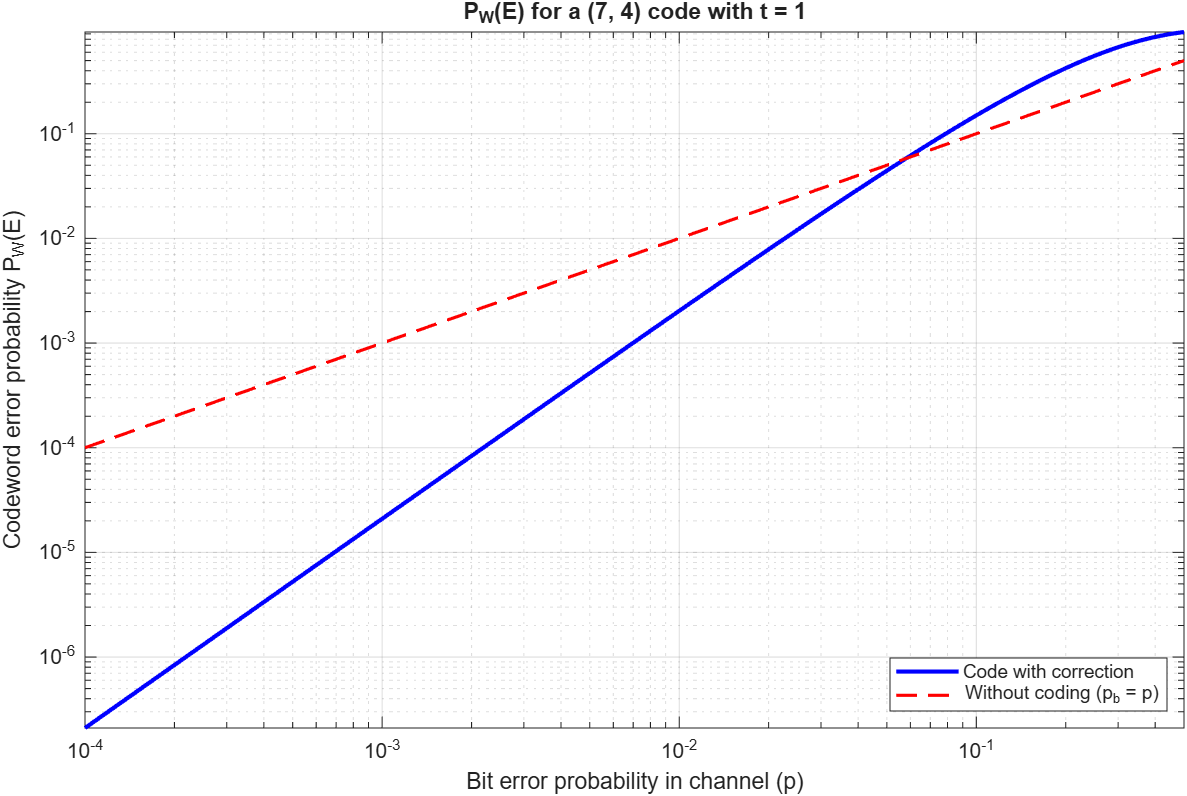
\includegraphics[width=0.72\textwidth, height=4.5cm, keepaspectratio]{A1_E4a.png}
\end{frame}

\begin{frame}[plain]
  \vfill
  \centering
  {\color{TealAccent}\rule{2cm}{2pt}}\\[0.4cm]
  {\LARGE\bfseries\color{NavyPrimary} Exercise 4b}\\[0.2cm]
  {\large\color{SlateNeutral} Simulation}
  \vfill
\end{frame}

\begin{frame}{Exercise 4b}
  \question{2. Explain why you focused on this region of the curve.}

  \vspace{0.25cm}
  \begin{itemize}
    \item We focused on the interval $p \in [0.06, 0.10]$ because for smaller values of $p$ the word error probability $P_W(E)$ drops very quickly ($\propto p^2$).
    \item Since the number of simulated codewords needed to observe $N_e$ errors scales as $N_e / P_W(E)$, collecting 100 word errors at $p = 0.06$ ($P_W(E) \approx 0.064$) takes around $1.56 \times 10^3$ transmissions, whereas at $p = 10^{-4}$ ($P_W(E) \approx 2.1 \times 10^{-7}$) it would require almost $5 \times 10^8$ transmissions, making the simulation too slow.
    \item Moreover, around $p \approx 0.056$ the $P_W(E)$ curve crosses the uncoded reference $p_b = p$, so this region shows both the transition where coding becomes advantageous and the theoretical $\propto p^2$ slope on a log-log plot.
  \end{itemize}
\end{frame}

\begin{frame}{Exercise 4b}
  \question{3. Plot the analytical and simulated curves on the same graph}

  \vspace{0.15cm}
  \begin{itemize}
    \item Comparison between the theoretical $P_W(E)$ curve and the Monte Carlo simulations with a stopping target of 10 and 100 word errors over $p \in [0.06, 0.10]$.
  \end{itemize}

  \vspace{0.1cm}
  \begin{center}
    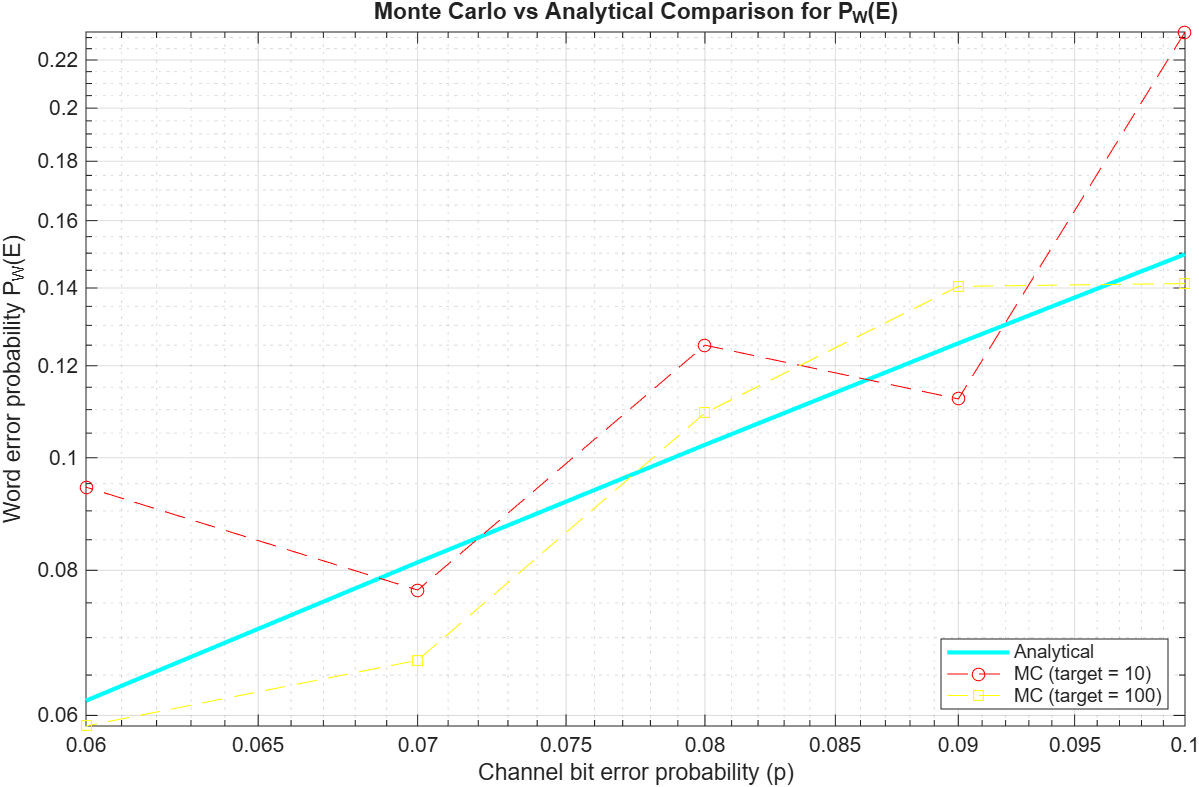
\includegraphics[width=0.72\textwidth, height=4.5cm, keepaspectratio]{A1_E4b.png}
  \end{center}
\end{frame}

\begin{frame}{Exercise 4b}
  \question{4. Comment on the results}

  \vspace{0.25cm}
  \begin{itemize}
    \item With a target of \textbf{10 word errors}, the simulated curve shows strong fluctuations around the analytical curve and is not even monotonic (e.g., jumping to $\approx 0.23$ at $p = 0.10$ and rising again at $p = 0.06$) because the sample size is too small to average out random channel noise.
    \item Increasing the target to \textbf{100 word errors} reduces the statistical variance by a factor of $10$, making the empirical curve much smoother and closely aligned with the theoretical curve across the whole interval.
    \item As $p$ decreases, $P_W(E)$ decreases following the theoretical $\propto p^2$ slope on the log-log plot, confirming that double-bit errors dominate in this regime.
    \item Overall, there is a direct trade-off between accuracy and simulation runtime: increasing the target from $10$ to $100$ errors yields a much more reliable estimate at the cost of $10\times$ more simulated transmissions.
  \end{itemize}
\end{frame}

\begin{frame}[plain]
  \vfill
  \centering
  {\color{TealAccent}\rule{2cm}{2pt}}\\[0.4cm]
  {\LARGE\bfseries\color{NavyPrimary} Exercise 4c}\\[0.2cm]
  {\large\color{SlateNeutral} Another (8,4) Code}
  \vfill
\end{frame}

\begin{frame}{Exercise 4c}
  \question{1. Determine the error-correction capability $t$ of the new code}

  \vspace{0.25cm}
  \begin{itemize}
    \item From the systematic generator matrix $G = [I_4 \mid A] \in \mathbb{F}_2^{4 \times 8}$, the code has parameters $n = 8$ and $k = 4$.
    \item The minimum Hamming weight among all non-zero codewords is $d_{\min} = 3$ (e.g., the third row of $G$, $0010\,0011$, has weight $3$).
    \item The error-correction capability is therefore:
    \[
      t = \left\lfloor \frac{d_{\min} - 1}{2} \right\rfloor = \frac{3 - 1}{2} = 1\text{ bit}
    \]
  \end{itemize}
\end{frame}

\begin{frame}{Exercise 4c}
  \question{2. Verify if it is perfect}

  \vspace{0.25cm}
  \begin{itemize}
    \item For $n = 8$ and $t = 1$, a Hamming sphere centered at each codeword contains:
    \[
      |S(c, 1)| = \binom{8}{0} + \binom{8}{1} = 1 + 8 = 9\text{ vectors}
    \]
    \item Multiplying by the $2^k = 2^4 = 16$ codewords gives:
    \[
      16 \times 9 = 144 \neq 2^8 = 256
    \]
    \item Since the Hamming bound does not hold with equality ($112$ vectors in $\mathbb{F}_2^8$ fall outside the spheres of radius $1$), \textbf{this $(8,4)$ code is not perfect}.
  \end{itemize}
\end{frame}

\begin{frame}{Exercise 4c}
  \question{3. Derive analytically $P_W(E)$.}

  \vspace{0.25cm}
  \begin{itemize}
    \item With bounded-distance decoding ($t = 1$), the decoder corrects error patterns of weight $0$ or $1$, so the probability of correct decoding is:
    \[
      P_W(C) = (1 - p)^8 + 8p(1 - p)^7
    \]
    \item Therefore, the word error probability is:
    \[
      P_W(E) = 1 - P_W(C) = 1 - (1 - p)^8 - 8p(1 - p)^7 = \sum_{w=2}^{8} \binom{8}{w} p^w (1 - p)^{8 - w}
    \]
    \item Since the code is not perfect, this formula is exact only for bounded-distance decoding (which corrects up to $t=1$ error), while under complete minimum-distance decoding some weight-$2$ errors could also be corrected.
  \end{itemize}
\end{frame}

\begin{frame}{Exercise 4c}
  \question{5. Compare the results obtained for the two codes and comment on any differences.}

  \vspace{0.25cm}
  \begin{itemize}
    \item Both codes have $k = 4$, $d_{\min} = 3$, and $t = 1$, but the $(8,4)$ code uses an extra parity bit ($n = 8$ instead of $n = 7$), lowering the code rate from $R = 4/7 \approx 0.57$ to $R = 4/8 = 0.5$.
    \item Since $n$ is larger while $t = 1$ stays the same, there are more double-bit error combinations ($\binom{8}{2} = 28$ vs. $\binom{7}{2} = 21$), so the $(8,4)$ code has a slightly higher word error probability ($P_W(E) \approx 28p^2$ vs. $\approx 21p^2$ for small $p$).
    \item Unlike the Hamming $(7,4)$ code, which is perfect ($16 \times 8 = 128 = 2^7$), the $(8,4)$ code is not perfect ($16 \times 9 = 144 < 256$), leaving $112$ vectors outside the Hamming spheres of radius $1$.
  \end{itemize}
\end{frame}

% ==============================================================================
% EXERCISE 5.1: Syndrome Decoding
% ==============================================================================
\begin{frame}[plain]
  \vfill
  \centering
  {\color{TealAccent}\rule{2cm}{2pt}}\\[0.4cm]
  {\LARGE\bfseries\color{NavyPrimary} Exercise 5.1}\\[0.2cm]
  {\large\color{SlateNeutral} Syndrome Decoding}
  \vfill
\end{frame}

\begin{frame}{Exercise 5.1 - Question 2}
	\question{2. Derive and plot the analytical codeword error probability $P_W(p)$ for $p \in [10^{-3}, 10^{-1}]$.}
	
	\vspace{0.15cm}
	\begin{columns}[c]
		\begin{column}{0.52\textwidth}
			\footnotesize
			\begin{itemize}
				\item The $(63, 57)$ binary Hamming code has $d_{\min} = 3$, so it corrects up to $t = \lfloor (d_{\min}-1)/2 \rfloor = 1$ bit error per codeword.
				\item A codeword error occurs whenever 2 or more bit errors happen over $n = 63$ bits:
				\[
				P_W(p) = 1 - (1-p)^{63} - 63\,p(1-p)^{62}
				\]
				\item For small $p$ ($p \approx 10^{-3}$), $P_W(p) \approx \binom{63}{2} p^2 = 1953\,p^2 \approx 1.95 \times 10^{-3}$.
				\item As $p$ approaches $10^{-1}$, multiple errors become dominant and $P_W(p)$ rises steeply toward $1$ ($P_W(0.1) \approx 0.99$).
			\end{itemize}
		\end{column}
		\begin{column}{0.45\textwidth}
			\centering
			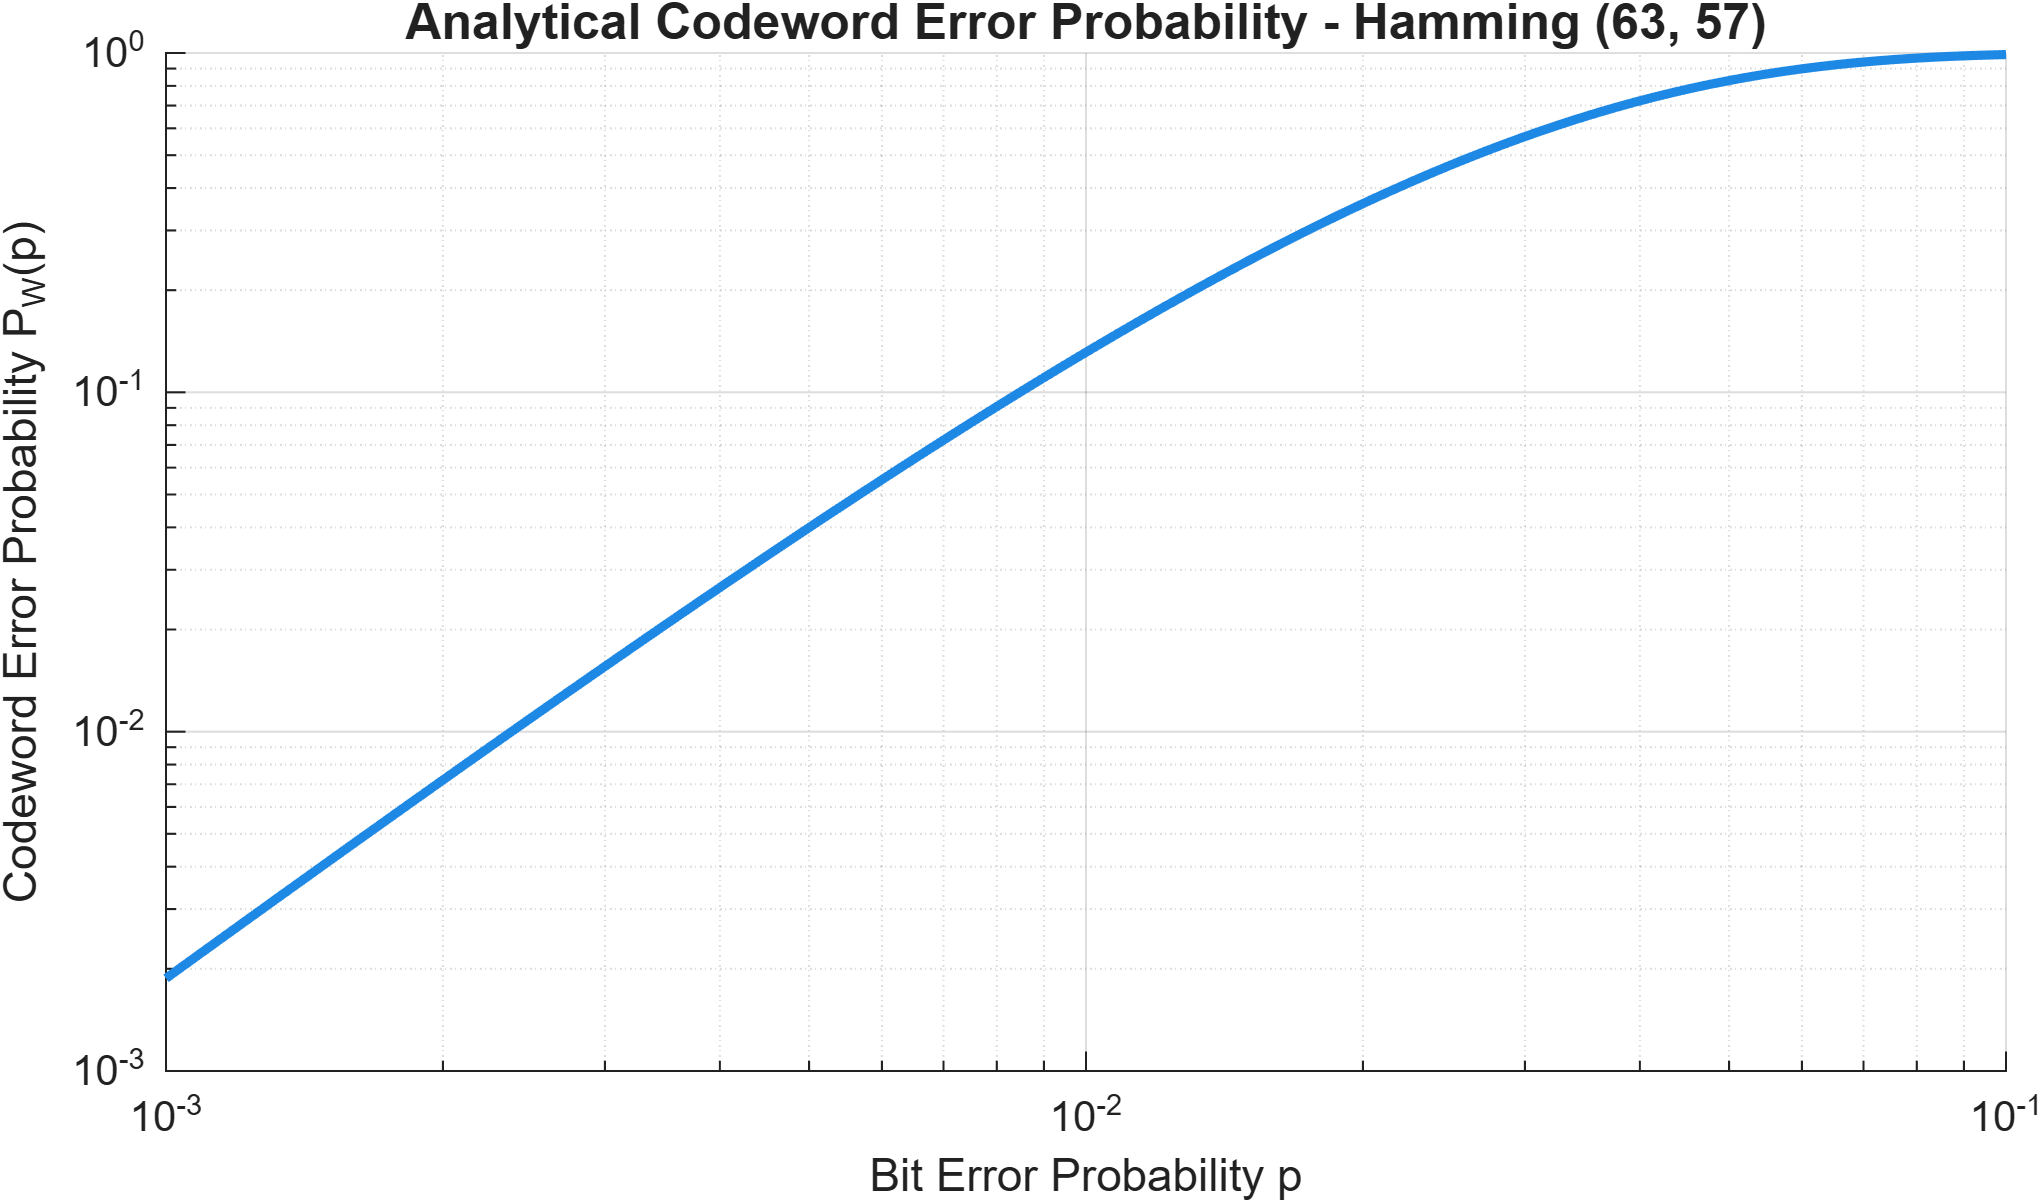
\includegraphics[width=\textwidth, height=4.4cm, keepaspectratio]{E5_1_Q2.png}
		\end{column}
	\end{columns}
\end{frame}

\begin{frame}{Exercise 5.1 - Question 3}
	\question{3. Simulate the bounded-distance decoder over the BSC for 8 values of $p \in [10^{-3}, 10^{-1}]$ (stopping at 100 codeword errors per point) and plot the estimated $\hat{P}_W(p)$.}
	
	\vspace{0.15cm}
	\begin{columns}[c]
		\begin{column}{0.52\textwidth}
			\footnotesize
			\begin{itemize}
				\item For each of the 8 logarithmically spaced values of $p$, random codewords $c = uG \bmod 2$ are transmitted over a BSC until 100 decoding errors occur.
				\item At the receiver, the syndrome $s = yH^T \bmod 2$ is computed:
				\begin{itemize}
					\item if $s = 0$, no error is assumed;
					\item if $s \neq 0$, the bit corresponding to the matching column of $H$ is flipped.
				\end{itemize}
				\item A codeword error is counted whenever $\hat{c} \neq c$, yielding the Monte Carlo estimate $\hat{P}_W(p) = 100 / N_{\text{words}}$.
				\item Stopping at 100 errors ensures a consistent relative confidence interval across all simulated points, even at low $p$.
			\end{itemize}
		\end{column}
		\begin{column}{0.45\textwidth}
			\centering
			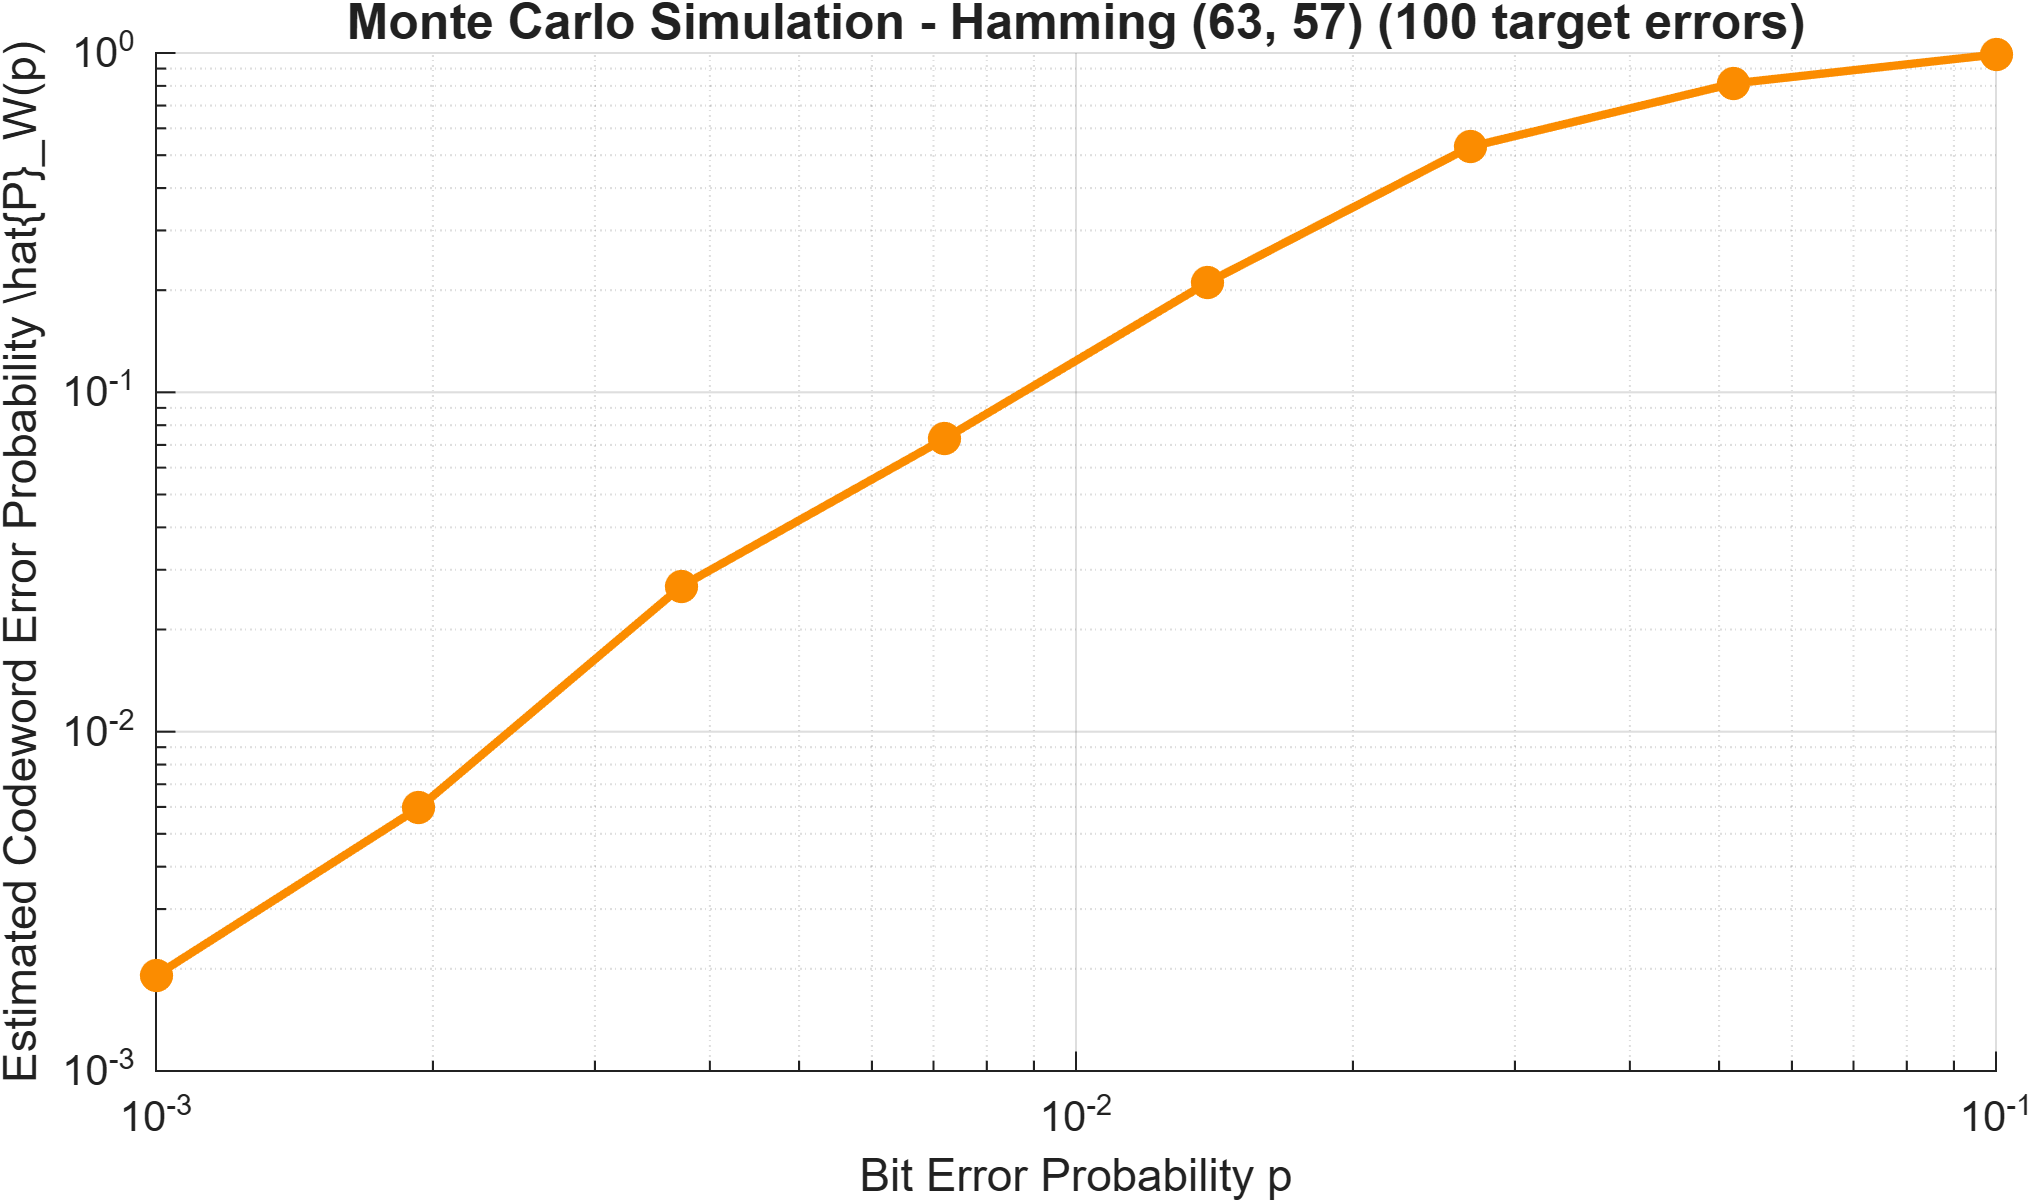
\includegraphics[width=\textwidth, height=4.4cm, keepaspectratio]{E5_1_Q3.png}
		\end{column}
	\end{columns}
\end{frame}

\begin{frame}{Exercise 5.1 - Question 5}
	\question{5. Compare the performance of the bounded-distance decoder with that of a complete minimum-distance decoder for this code.}
	
	\vspace{0.15cm}
	\begin{columns}[c]
		\begin{column}{0.52\textwidth}
			\footnotesize
			\begin{itemize}
				\item The $(63, 57)$ binary Hamming code is a perfect code: the $2^{57}$ disjoint Hamming spheres of radius $t = 1$, each containing $1 + 63 = 2^6$ vectors, completely partition $\{0,1\}^{63}$ ($2^{57} \cdot 2^6 = 2^{63}$).
				\item Every possible $6$-bit syndrome maps uniquely to an error pattern of weight $w \le 1$, so no received vector ever falls outside the decoding spheres and decoding failures never occur.
				\item Thus, the bounded-distance decoder is identical to a complete minimum-distance decoder, as confirmed by the exact overlap between the simulated curve and the analytical bound.
			\end{itemize}
		\end{column}
		\begin{column}{0.45\textwidth}
			\centering
			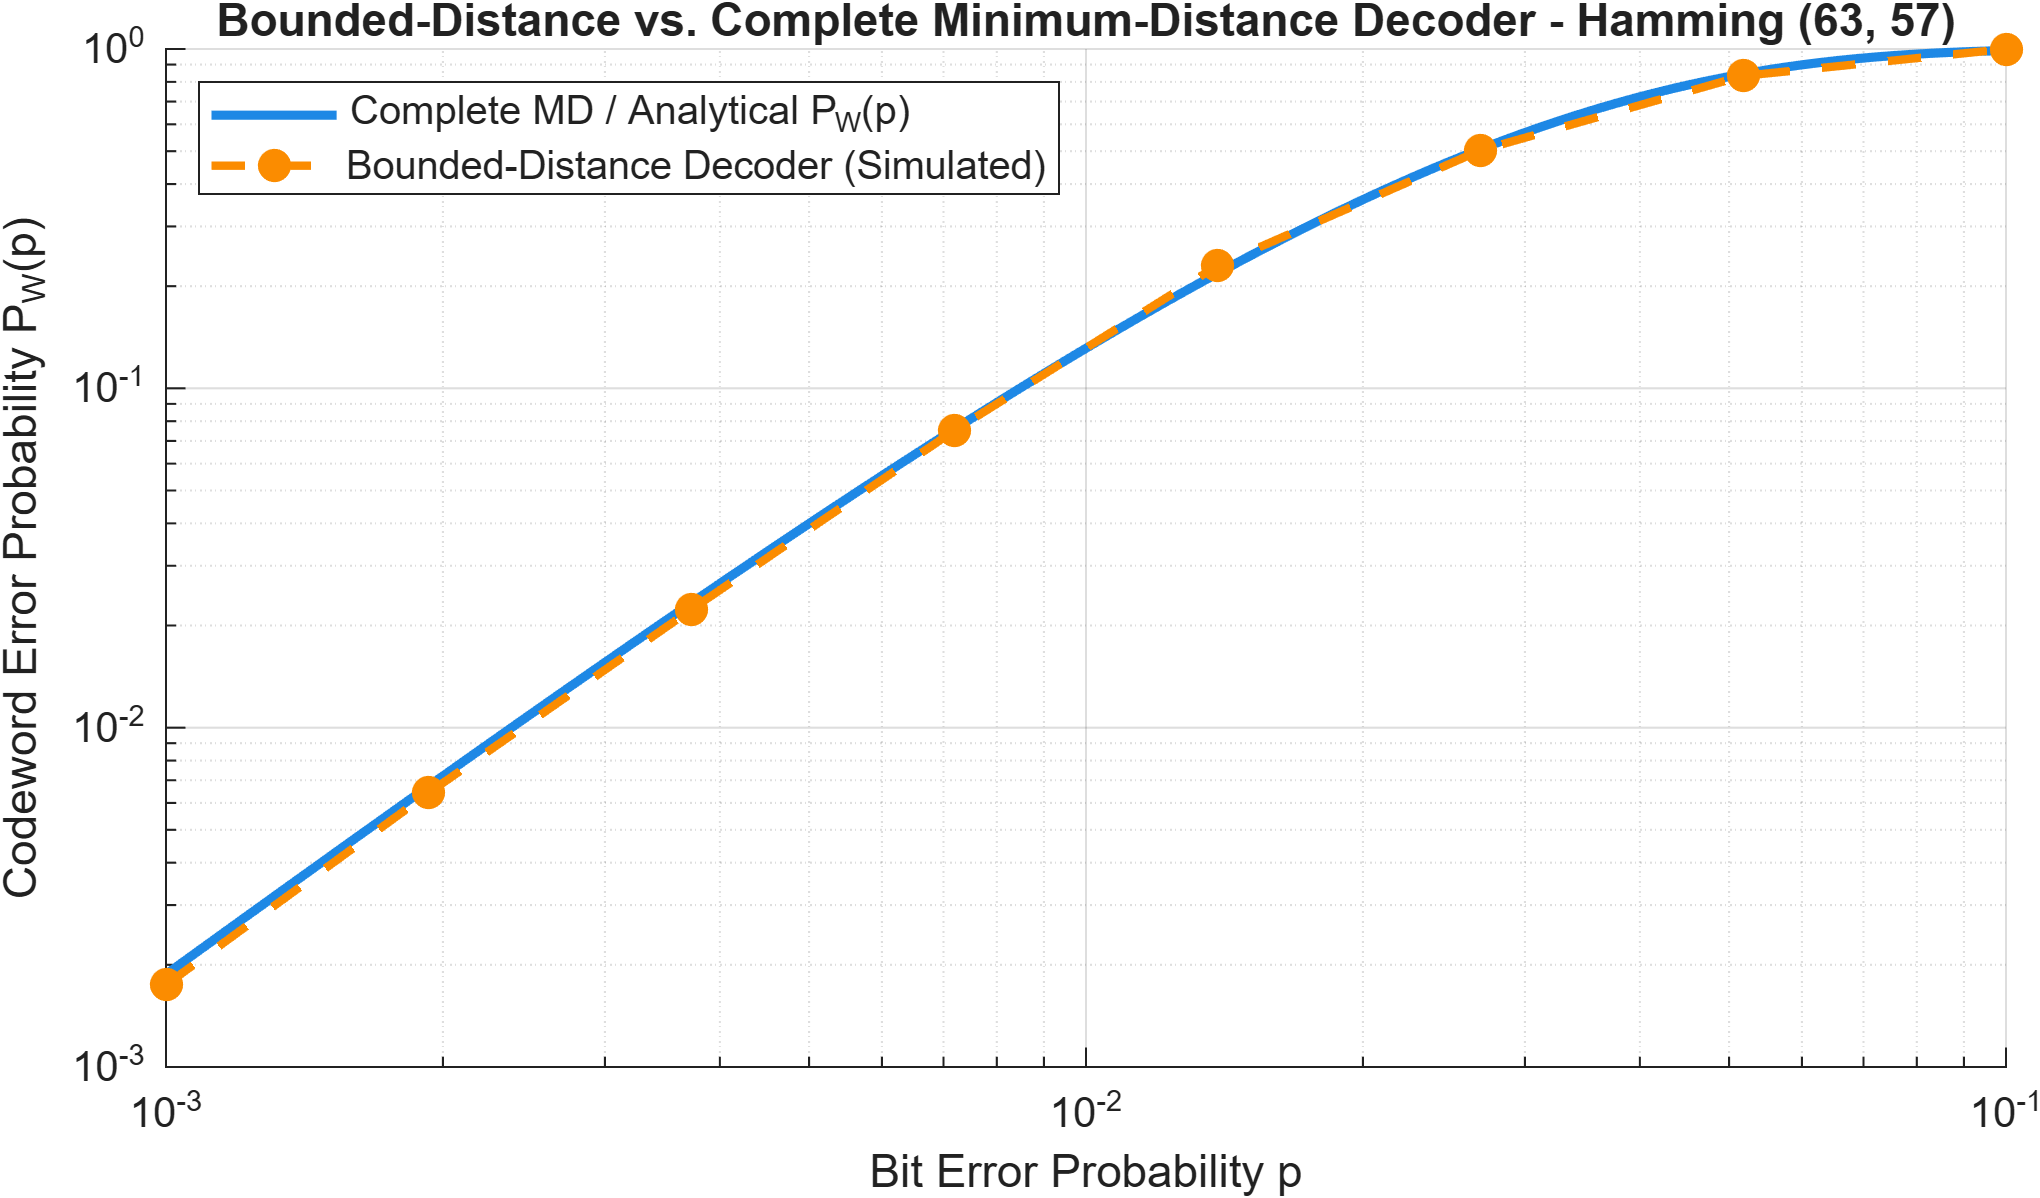
\includegraphics[width=\textwidth, height=4.4cm, keepaspectratio]{E5_1_Q5.png}
		\end{column}
	\end{columns}
\end{frame}

\begin{frame}{Exercise 5.1 - Question 7}
	\question{7. Discuss how changing $(n, k)$ affects error-correction capability and code rate, and whether any $(n, k)$ pair can be chosen for a binary Hamming code.}
	
	\vspace{0.2cm}
	\begin{itemize}
		\item No: a binary Hamming code cannot have an arbitrary $(n, k)$ pair. Its parameters are strictly constrained to $(n, k) = (2^r - 1,\, 2^r - 1 - r)$ for an integer $r \ge 3$.
		\item Every binary Hamming code has $d_{\min} = 3$, meaning its error-correction capability is always fixed at $t = 1$ bit error per codeword regardless of $r$ (to achieve $t > 1$, other code families such as BCH codes are required).
		\item Increasing $r$ raises the code rate $R = k/n = 1 - \frac{r}{2^r - 1}$ (less redundancy overhead), but since $t = 1$ remains fixed over a longer block $n$, multiple errors become more likely and $P_W(p) \approx \binom{n}{2}p^2$ degrades.
	\end{itemize}
\end{frame}

% ==============================================================================
% EXERCISE 6: Properties of m-sequences
% ==============================================================================
\begin{frame}[plain]
  \vfill
  \centering
  {\color{TealAccent}\rule{2cm}{2pt}}\\[0.4cm]
  {\LARGE\bfseries\color{NavyPrimary} Exercise 6}\\[0.2cm]
  {\large\color{SlateNeutral} Properties of m-sequences}
  \vfill
\end{frame}

\begin{frame}{Exercise 6 - Sequence}
  \question{1. Choose a random seed and write it.}
\end{frame}

\begin{frame}{Exercise 6 - Sequence}
  \question{3. Plot the first 20 bits of the bipolar sequence ($0 \to -1$ and $1 \to +1$)}
\end{frame}

\begin{frame}{Exercise 6 - Sequence}
  \question{3. Comment the result.}
\end{frame}

\begin{frame}{Exercise 6 - Number of zero/ones, number of transitions}
  \question{1. Write a table with $N_1$ and $N_0$ (number of bits equal to 1 and 0), $N_T$ and $N_{NT}$ (number of transitions and no transitions, view the sequence as periodic).}
\end{frame}

\begin{frame}{Exercise 6 - Number of zero/ones, number of transitions}
  \question{2. Check if the properties of an ideal binary sequences are verified and discuss the result}
\end{frame}

\begin{frame}{Exercise 6 - Runs}
  \question{1. Write a table with the values of $N_R(T)$ (total number of runs), $N_R(i)$ (number of runs of length $i$), $N_{R0}(i)$ and $N_{R1}(i)$ (number of runs of zeros and ones of length $i$)}
\end{frame}

\begin{frame}{Exercise 6 - Runs}
  \question{2. Plot the run lengths vs. their starting point in the sequence (use different colors for 0 and 1 runs)}
\end{frame}

\begin{frame}{Exercise 6 - Runs}
  \question{3. Compare against the run properties of an ideal binary random sequence and discuss the results.}
\end{frame}

\begin{frame}{Exercise 6 - Autocorrelation}
  \question{1. Plot the autocorrelation}
\end{frame}

\begin{frame}{Exercise 6 - Autocorrelation}
  \question{2. Compare its properties with those of an ideal binary random sequences.}
\end{frame}

\begin{frame}{Exercise 6 - Truncated sequences - MPSL}
  \question{5. Plot $MPSL(z)$ vs. $z$}
\end{frame}

\begin{frame}{Exercise 6 - Truncated sequences - MPSL}
  \question{6. Comment the results}
\end{frame}

\begin{frame}{Exercise 6 - Truncated sequences - seed}
  \question{4. Plot it}
\end{frame}

\begin{frame}{Exercise 6 - Truncated sequences - seed}
  \question{5. Repeat and plot with the same $z$ but another starting seed}
\end{frame}

\begin{frame}{Exercise 6 - Truncated sequences - seed}
  \question{6. Comment the results}
\end{frame}

% Slide finale
\begin{frame}[plain]
  \vfill
  \centering
  {\color{TealAccent}\rule{2.5cm}{2pt}}\\[0.5cm]
  {\Huge\bfseries\color{NavyPrimary} Grazie!}\\[0.3cm]
  \vfill
\end{frame}

\end{document}